% !TeX program = xelatex
% !TeX TXS-program:compile = txs:///xelatex/[--shell-escape]
%%%%%%%%%%%%%%%%%%%%%%%%%%%%%%%%%%%%%%%%%%%%%%%%%%%%%%%%%%%%%%%%%%%%%%%%
% Plantilla TFG/TFM
% Escuela Politécnica Superior de la Universidad de Alicante
% Realizado por: Jose Manuel Requena Plens
% Contacto: info@jmrplens.com / Telegram:@jmrplens
%%%%%%%%%%%%%%%%%%%%%%%%%%%%%%%%%%%%%%%%%%%%%%%%%%%%%%%%%%%%%%%%%%%%%%%%

% Elige si deseas optimizar la ejecución del proyecto almacenando las figuras generadas con TikZ y PGF en una carpeta (archivos/figuras-procesadas).
% 1 - Si, 2 - No
\def\OptimizaTikZ{1}

% Archivo .TEX que incluye todas las configuraciones del documento y los paquetes. Añade todo aquello que necesites utilizar en el documento en este archivo.
% En él se encuentra la configuración de los márgenes, establecidos según las directrices de estilo de la EPS.
%%%%%%%%%%%%%%%%%%%%%%%%%%%%%%%%%%%%%%%%%%%%%%%%%%%%%%%%%%%%%%%%%%%%%%%%
% Plantilla TFG/TFM
% Escuela Politécnica Superior de la Universidad de Alicante
% Realizado por: Jose Manuel Requena Plens
% Contacto: info@jmrplens.com / Telegram:@jmrplens
%%%%%%%%%%%%%%%%%%%%%%%%%%%%%%%%%%%%%%%%%%%%%%%%%%%%%%%%%%%%%%%%%%%%%%%%

%%%%%%%%%%%%%%%%%%%%%%%%
% FORMATO DEL DOCUMENTO
%%%%%%%%%%%%%%%%%%%%%%%%
% scrbook es la clase de documento
% Si se desea que no haya página en blanco entre capítulos añadir "openany" en los parámetros de la clase. Sino siempre los capítulos empezarán en página impar.
\documentclass[a4paper,11pt,titlepage]{scrbook}
\KOMAoption{toc}{bib,chapterentryfill} % Opciones del índice
\usepackage{scrhack} % Previene algunos errores
% Paquete de formato para scrbook. Con marcas, linea-separador superior e inferior
\usepackage[automark,headsepline,footsepline]{scrlayer-scrpage}
\clearpairofpagestyles		% Borra los estilos por defecto
%%
% Formato y contenido de la información de cabecera y pie de página
%%
% Información de capítulo en cabecera e interno
\ihead{{\color{gray30}\scshape\small\headmark}}	
% Número de página en cabecera y externo
\ohead{\normalfont\pagemark} 
% Número de página en pie de página y externo. Sólo en páginas sin cabecera
\ofoot[\normalfont\pagemark]{}
%% 		
% Edición del contenido de las distintas partes de la cabecera
%%

\renewcommand{\sectionmark}[1]{\markright{\thesection. #1}} % Sección (Número y texto)
\setkomafont{pagenumber}{} % Número de página (Sin nada añadido)

% Añade al índice y numera hasta la profundidad 4.
% 1:section,2:subsection,3:subsubsection,4:paragraph
\setcounter{tocdepth}{4}
\setcounter{secnumdepth}{4}
% Muestra una regla para comprobar el formato de las páginas
%\usepackage[type=upperleft,showframe,marklength=8mm]{fgruler}
% MÁRGENES DE LAS PÁGINAS
\usepackage[
  inner	=	3.0cm, % Margen interior
  outer	=	2.5cm, % Margen exterior
  top	=	2.5cm, % Margen superior
  bottom=	2.5cm, % Margen inferior
  includeheadfoot, % Incluye cabecera y pie de página en los márgenes
]{geometry}
% Valor de interlineado
\renewcommand{\baselinestretch}{1.0} % 1 línea de interlineado
% Para poder generar páginas horizontales
\usepackage{lscape}
% Ancho de la zona para comentarios en el margen. (modificado para todonotes)
\setlength{\marginparwidth}{2cm}

%%%%%%%%%%%%%%%%%%%%%%%%
% BIBLIOGRAFÍA
%%%%%%%%%%%%%%%%%%%%%%%%
\usepackage{apacite} % NORMA APA
\usepackage{natbib}
\usepackage{breakcites}

%%%%%%%%%%%%%%%%%%%%%%%%
% DOCUMENTO EN ESPAÑOL
%%%%%%%%%%%%%%%%%%%%%%%%
\usepackage[base]{babel}
\usepackage{polyglossia}
\setdefaultlanguage{spanish}

\addto\captionsspanish{%
	\renewcommand{\listtablename}{Índice de tablas} 
	\renewcommand{\tablename}{Tabla}
	\renewcommand{\lstlistingname}{Código}
	\renewcommand{\lstlistlistingname}{Índice de \lstlistingname s}
	\renewcommand{\glossaryname}{Glosario}
	\renewcommand{\acronymname}{Acrónimos}
	\renewcommand{\bibname}{Bibliografía}%
}

%%%%%%%%%%%%%%%%%%%%%%%% 
% COLORES
%%%%%%%%%%%%%%%%%%%%%%%% 
% Biblioteca de colores
\usepackage{color}
\usepackage[dvipsnames]{xcolor}
% Otros colores definidos por el usuario
\definecolor{gray97}{gray}{.97}
\definecolor{gray75}{gray}{.75}
\definecolor{gray45}{gray}{.45}
\definecolor{gray30}{gray}{.30}
\definecolor{negro}{RGB}{0,0,0}
\definecolor{blanco}{RGB}{255,255,255}
\definecolor{dkgreen}{rgb}{0,.6,0}
\definecolor{dkblue}{rgb}{0,0,.6}
\definecolor{dkyellow}{cmyk}{0,0,.8,.3}
\definecolor{gray}{rgb}{0.5,0.5,0.5}
\definecolor{mauve}{rgb}{0.58,0,0.82}
\definecolor{deepblue}{rgb}{0,0,0.5}
\definecolor{deepred}{rgb}{0.6,0,0}
\definecolor{deepgreen}{rgb}{0,0.5,0}
\definecolor{MyDarkGreen}{rgb}{0.0,0.4,0.0}
\definecolor{bluekeywords}{rgb}{0.13,0.13,1}
\definecolor{greencomments}{rgb}{0,0.5,0}
\definecolor{redstrings}{rgb}{0.9,0,0}

%%%%%%%%%%%%%%%%%%%%%%%%
% TABLAS
%%%%%%%%%%%%%%%%%%%%%%%%
% Paquetes para tablas
\usepackage{longtable,booktabs,array,multirow,multicol,tabularx,ragged2e,array}
% Nuevos tipos de columna para tabla, se pueden utilizar como por ejemplo C{3cm} en la definición de columnas de la función tabular
\newcolumntype{L}[1]{>{\raggedright\let\newline\\\arraybackslash\hspace{0pt}}m{#1}}
\newcolumntype{C}[1]{>{\centering\let\newline\\\arraybackslash\hspace{0pt}}m{#1}}
\newcolumntype{R}[1]{>{\raggedleft\let\newline\\\arraybackslash\hspace{0pt}}m{#1}}

%%%%%%%%%%%%%%%%%%%%%%%% 
% GRAFICAS y DIAGRAMAS 
%%%%%%%%%%%%%%%%%%%%%%%% 
% Paquete para todo tipo de gráficas, diagramas, modificación de imágenes, etc
\usepackage{tikz,tikzpagenodes}
\usetikzlibrary{tikzmark,calc,shapes.geometric,arrows,backgrounds,shadings,shapes.arrows,shapes.symbols,shadows,positioning,fit,automata,patterns,intersections}
\usepackage{pgfplots}
\pgfplotsset{colormap/jet}
\pgfplotsset{compat=newest} % Compatibilidad
\usepgfplotslibrary{patchplots,groupplots,fillbetween,polar}
\usepackage{pgfplotstable}
% Guardar las figuras realizadas con Tikz y Pgf en una carpeta externa
% para agilizar el procesado y tenerlas para utilizarlas en otros
% documentos
\if\OptimizaTikZ 1
\usepgfplotslibrary{external}
\tikzexternalize[prefix=archivos/figuras-procesadas/] % Ruta
\tikzset{%
    external/system call ={xelatex -enable-write18 -halt-on-error -interaction=batchmode -jobname "\image" "\texsource"},
}
\fi

% Estilos para elementos graficos
% Cajas y cajas de texto
\tikzstyle{Caja1} = [green,very thick,rounded corners,fill=white, fill opacity=0.5]
\tikzstyle{Texto1} = [fill=white,thick,shape=circle,draw=black,inner sep=2pt,font=\sffamily,text=black]
\tikzstyle{Texto2} = [fill=white,thick,shape=rectangle,draw=black,inner sep=2pt,font=\sffamily,text=black]
\tikzstyle{Texto3} = [fill=white,thick,shape=circle,draw=black,inner sep=2pt,font=\sffamily,text=black]
% Cuadros de diagrama
\tikzstyle{rectvioleta} = [rectangle, rounded corners, text centered, draw=black, fill=blue!10]
\tikzstyle{rectnaranja} = [rectangle, minimum width=2cm, minimum height=1cm, text centered, draw=black, fill=orange!10]
\tikzstyle{romborosa} = [diamond, aspect=3, minimum width=3cm, minimum height=1cm, text centered, draw=black, fill=red!10]
\tikzstyle{rectverde} = [rectangle, minimum width=2cm, minimum height=1cm, text centered, draw=black, fill=green!10]
\tikzstyle{rectamarillo} = [rectangle, rounded corners, minimum width=2cm, minimum height=1cm, text centered, draw=black, fill=yellow!10]
% Flechas
\tikzstyle{arrow} = [thick,->,>=stealth]

%%%%%%%%%%%%%%%%%%%%%%%% 
% FIGURAS, TABLAS, ETC 
%%%%%%%%%%%%%%%%%%%%%%%% 
\usepackage{subcaption} % Para poder realizar subfiguras
\usepackage{caption} % Para aumentar las opciones de diseño
% Nombres de figuras, tablas, etc, en negrita la numeración, todo con letra small
\captionsetup{labelfont={bf,small},textfont=small}
% Paquete para modificar los espacios arriba y abajo de una figura o tabla
\usepackage{setspace}
% Define el espacio tanto arriba como abajo de las figuras, tablas
\setlength{\intextsep}{5mm}
% Para ajustar tamaños de texto de toda una tabla o grafica
% Uso: {\scalefont{0.8} \begin{...} \end{...} }
\usepackage{scalefnt}
% Redefine las tablas y figuras para eliminar el '.' entre la numeración y el texto
\renewcommand*{\figureformat}{\figurename~\thefigure}
\renewcommand*{\tableformat}{\tablename~\thetable}

%%%%%%%%%%%%%%%%%%%%%%%% 
% TEXTO
%%%%%%%%%%%%%%%%%%%%%%%%
% Paquete para poder modificar las fuente de texto
\usepackage{xltxtra}
% Cualquier tamaño de texto. Uso: {\fontsize{100pt}{120pt}\selectfont tutexto}
\usepackage{anyfontsize}
% Para modificar parametros del texto.
\usepackage{setspace}
% Paquete para posicionar bloques de texto
\usepackage{textpos}
% Paquete para realizar cajas de texto. 
% Uso: \begin{mdframed}[linecolor=red!100!black] tutexto \end{mdframed}
\usepackage{framed,mdframed}
% Para subrayar. Uso: \hlc[tucolor]{tutexto}
\newcommand{\hlc}[2][yellow]{ {\sethlcolor{#1} \hl{#2}} }

%%%%%%%%%%%%%%%%%%%%%%%% 
% OTROS
%%%%%%%%%%%%%%%%%%%%%%%%
% Para hacer una pagina horizontal. Uso: \begin{landscape} xxxx \end{lanscape}
\usepackage{lscape} 
% Para incluir paginas PDF. Uso:
% \includepdf[pages={1}]{tuarchivo.pdf}
\usepackage{pdfpages}
% Para introducir url's con formato. Uso: \url{http://www.google.es}
\usepackage{url}
% Amplia muchas funciones graficas de latex
\usepackage{graphicx}
% Paquete que añade el hipervinculo en referencias dentro del documento, indice, etc
% Se define sin bordes alrededor. Uso: \ref{tulabel}
\usepackage[pdfborder={000}]{hyperref}
\usepackage{float}
\usepackage{placeins}
\usepackage{afterpage}
\usepackage{verbatim}
% Paquete para condicionales avanzados
\usepackage{xstring,xifthen}
% Paquete para realizar calculos en el código
\usepackage{calc}
% Para rotar tablas o figuras o su contenido
\usepackage{rotating} 
% Para incluir comentarios en el texto. El parámetro 'disable' oculta todas las notas.
% USO: \todo{tutexto}
\usepackage[textsize=tiny,spanish,shadow,textwidth=2cm]{todonotes}
%\reversemarginpar % Descomentar si se quiere todos los comentarios en el mismo lado
% Desactiva la exportación de los ToDo y Missingfigures como figuras
\if\OptimizaTikZ 1
\makeatletter
\renewcommand{\todo}[2][]{\tikzexternaldisable\@todo[#1]{#2}\tikzexternalenable}
\makeatother
\usepackage{letltxmacro}
\LetLtxMacro{\oldmissingfigure}{\missingfigure}
\makeatletter
\renewcommand{\missingfigure}[2][]{\tikzexternaldisable\oldmissingfigure[{#1}]{#2}\tikzexternalenable}
\makeatother
\fi

%%%%%%%%%%%%%%%%%%%%%%%% 
% GLOSARIOS
%%%%%%%%%%%%%%%%%%%%%%%%
\usepackage[acronym,nonumberlist,toc]{glossaries}
\usepackage{glossary-superragged}
\newglossarystyle{modsuper}{%
  \setglossarystyle{super}%
  \renewcommand{\glsgroupskip}{}
}
\renewcommand{\glsnamefont}[1]{\textbf{#1}}


%%%%%%%%%%%%%%%%%%%%%%%% 
% COMANDOS AÑADIDOS
%%%%%%%%%%%%%%%%%%%%%%%%
% Para mostrar la fecha actual (mes año) con \Hoy
\newcommand{\MES}{%
  \ifcase\month% 0
    \or Enero% 1
    \or Febrero% 2
    \or Marzo% 3
    \or Abril% 4
    \or Mayo% 5
    \or Junio% 6
    \or Julio% 7
    \or Agosto% 8
    \or Septiembre% 9
    \or Octubre% 10
    \or Noviembre% 11
    \or Diciembre% 12
  \fi}
\newcommand{\ANYO}{\number\year}
\newcommand{\Hoy}{\MES\ \ANYO}

%%%%%%%%%%%%%%%%%%%%%%%% 
% MATEMÁTICAS
%%%%%%%%%%%%%%%%%%%%%%%%
\usepackage{mathtools,amsthm,amsfonts,amssymb,bm,mathrsfs,nicefrac,upgreek,bigints} 
% Comando para añadir información de variables a las ecuaciones
% Uso: \begin{condiciones}[donde:] ....... \end{condiciones}
\newenvironment{condiciones}[1][2]
  {%
   #1\tabularx{\textwidth-\widthof{#1}}[t]{
     >{$}l<{$} @{}>{${}}c<{{}$}@{} >{\raggedright\arraybackslash}X
   }%
  }
  {\endtabularx\\[\belowdisplayskip]}

%%%%%
% PARÁMETROS DE FORMATO DE CODIGOS
%%%%%
% Puedes editar los formatos para ajustarlos a tu gusto
%%%%%%%%%%%%%%%%%%%%%%%%%%%%%%%%%%%%%%%%%%%%%%%%%%%%%%%%%%%%%%%%%%%%%%%%
% Plantilla TFG/TFM
% Escuela Politécnica Superior de la Universidad de Alicante
% Realizado por: Jose Manuel Requena Plens
% Contacto: info@jmrplens.com / Telegram:@jmrplens
%%%%%%%%%%%%%%%%%%%%%%%%%%%%%%%%%%%%%%%%%%%%%%%%%%%%%%%%%%%%%%%%%%%%%%%%


%%%%%%%%%%%%%%%%%%%%%%%% 
% CÓDIGO. CONFIGURACIÓN. En el siguiente bloque están los estilos.
%%%%%%%%%%%%%%%%%%%%%%%%
% Paquete para mostrar código de matlab. En caja y lineas numeradas
\usepackage[framed,numbered]{matlab-prettifier}
% Paquete mostrar código de programación de distintos lenguajes
\usepackage{listings}
\lstset{ inputencoding=utf8,
extendedchars=true,
%frame=single, % Caja donde se ubica el código
%backgroundcolor=\color{white}, % Color del fondo de la caja
rulesepcolor=\color{black},
boxpos=c,
abovecaptionskip=-4pt,
aboveskip=12pt,
belowskip=0pt,
lineskip=0pt,
framerule=0pt,
framextopmargin=4pt,
framexbottommargin=4pt,
framexleftmargin=11pt,
framexrightmargin=0pt,
linewidth=\linewidth,
xleftmargin=\parindent,
framesep=0pt,
rulesep=.4pt,
stringstyle=\ttfamily,
showstringspaces = false,
showspaces = false,
showtabs = false,
columns=fullflexible,
basicstyle=\small\ttfamily,
commentstyle=\color{gray45},
keywordstyle=\bfseries,
tabsize=4,
numbers=left,
numbersep=1pt,
numberstyle=\tiny\ttfamily\color{gray75},
numberfirstline = false,
breaklines=true,
postbreak=\mbox{\textcolor{red}{$\hookrightarrow$}\space}, % Flecha al saltar de linea
prebreak=\mbox{\textcolor{red}{$\hookleftarrow$}\space}, % Flecha al saltar de linea
literate=
  {á}{{\'a}}1 {é}{{\'e}}1 {í}{{\'i}}1 {ó}{{\'o}}1 {ú}{{\'u}}1
  {Á}{{\'A}}1 {É}{{\'E}}1 {Í}{{\'I}}1 {Ó}{{\'O}}1 {Ú}{{\'U}}1
  {à}{{\`a}}1 {è}{{\`e}}1 {ì}{{\`i}}1 {ò}{{\`o}}1 {ù}{{\`u}}1
  {À}{{\`A}}1 {È}{{\'E}}1 {Ì}{{\`I}}1 {Ò}{{\`O}}1 {Ù}{{\`U}}1
  {ä}{{\"a}}1 {ë}{{\"e}}1 {ï}{{\"i}}1 {ö}{{\"o}}1 {ü}{{\"u}}1
  {Ä}{{\"A}}1 {Ë}{{\"E}}1 {Ï}{{\"I}}1 {Ö}{{\"O}}1 {Ü}{{\"U}}1
  {â}{{\^a}}1 {ê}{{\^e}}1 {î}{{\^i}}1 {ô}{{\^o}}1 {û}{{\^u}}1
  {Â}{{\^A}}1 {Ê}{{\^E}}1 {Î}{{\^I}}1 {Ô}{{\^O}}1 {Û}{{\^U}}1
  {œ}{{\oe}}1 {Œ}{{\OE}}1 {æ}{{\ae}}1 {Æ}{{\AE}}1 {ß}{{\ss}}1
  {ű}{{\H{u}}}1 {Ű}{{\H{U}}}1 {ő}{{\H{o}}}1 {Ő}{{\H{O}}}1
  {ç}{{\c c}}1 {Ç}{{\c C}}1 {ø}{{\o}}1 {å}{{\r a}}1 {Å}{{\r A}}1
  {€}{{\euro}}1 {£}{{\pounds}}1 {«}{{\guillemotleft}}1
  {»}{{\guillemotright}}1 {ñ}{{\~n}}1 {Ñ}{{\~N}}1 {¿}{{?`}}1,
  }

% Intenta no dividir los códigos en diferentes paginas si es posible
\lstnewenvironment{listing}[1][]
   {\lstset{#1}\pagebreak[0]}{\pagebreak[0]}

% Formato de títulos de los códigos
\DeclareCaptionFont{white}{\color{white}}
\DeclareCaptionFormat{listing}{\colorbox{gray}{\parbox{\textwidth - 2\fboxsep}{#1#2#3}}}
\captionsetup[lstlisting]{format=listing,labelfont=white,textfont=white,font= scriptsize}


%%%%%%%%%%%%%%%%%%%%%%%% 
% CÓDIGO. ESTILOS. Ajústalos a tu gusto
%%%%%%%%%%%%%%%%%%%%%%%%
\lstdefinestyle{Consola}
	{
	basicstyle=\scriptsize\bfseries\ttfamily,
	}
   
\lstdefinestyle{C}
	{
	basicstyle=\scriptsize,
	language=C,
	}
\lstdefinestyle{C-color}
	{
  	breaklines=true,
  	language=C,
  	basicstyle=\scriptsize,
  	keywordstyle=\bfseries\color{green!40!black},
  	commentstyle=\itshape\color{purple!40!black},
  	identifierstyle=\color{blue},
  	stringstyle=\color{orange},
    }
\lstdefinestyle{CSharp}
	{
	basicstyle=\scriptsize,
	language=[Sharp]C,
	escapeinside={(*@}{@*)},
	keywordstyle=\bfseries,
	}
\lstdefinestyle{CSharp-color}
	{
	basicstyle=\scriptsize,
	language=[Sharp]C,
	escapeinside={(*@}{@*)},
	commentstyle=\color{greencomments},
	keywordstyle=\color{bluekeywords}\bfseries,
	stringstyle=\color{redstrings},
	}
\lstdefinestyle{C++}
	{
	basicstyle=\scriptsize,
	language=C++,
 	}
 	
\lstdefinestyle{C++-color}
	{
  	breaklines=true,
  	language=C++,
  	basicstyle=\scriptsize,
  	keywordstyle=\bfseries\color{green!40!black},
  	commentstyle=\itshape\color{purple!40!black},
  	identifierstyle=\color{blue},
  	stringstyle=\color{orange},
    }
    
\lstdefinestyle{PHP}
	{
	basicstyle=\scriptsize,
	language=PHP,
	}
	
\lstdefinestyle{PHP-color}
	{
	basicstyle=\scriptsize,
	language=PHP,
	keywordstyle    = \color{dkblue},
  	stringstyle     = \color{red},
  	identifierstyle = \color{dkgreen},
  	commentstyle    = \color{gray},
  	emph            =[1]{php},
  	emphstyle       =[1]\color{black},
  	emph            =[2]{if,and,or,else},
  	emphstyle       =[2]\color{dkyellow}
  }
  
\lstdefinestyle{Matlab}
	{
	basicstyle=\scriptsize,
	language=Matlab,
	numberstyle=\tiny\ttfamily\color{gray75},
	}
	
\lstdefinestyle{Matlab-color}
	{
	style = Matlab-editor,
	basicstyle=\scriptsize,
	numberstyle=\tiny\ttfamily\color{gray75},
	}
	
\lstdefinestyle{Latex}
	{
	language=[LaTeX]{Tex},
    basicstyle=\scriptsize,
    literate={\$}{{{\bfseries\$}}}1,
    alsoletter={\\,*,\&},
    emph =[1]{\\begin,\\end,\\caption,\\label,\\centering,\\FloatBarrier,
              \\lstinputlisting,\\scalefont,\\addplot,\\input,
              \\legend,\\item,\\subitem,\\includegraphics,\\textwidth,
              \\section,\\subsection,\\subsubsection,\\paragraph,
              \\cite,\\citet,\\citep,\\gls,\\bibliographystyle,\\url,
              \\citet*,\\citep*,\\todo,\\missingfigure,\\footnote},
  	emphstyle =[1]\bfseries,
  	emph = [2]{equation,subequations,eqnarray,figure,subfigure,
  			   condiciones,flalign,tikzpicture,axis,lstlisting,
  			   itemize,description
  			   },
  	emphstyle =[2]\bfseries,
    numbers=none,
	}
	
\lstdefinestyle{Latex-color}
	{
	language=[LaTeX]{Tex},
    basicstyle=\scriptsize,
    commentstyle=\color{dkgreen},
    identifierstyle=\color{black},
    literate={\$}{{{\bfseries\color{Dandelion}\$}}}1, % Colorea el simbolo dollar
    alsoletter={\\,*,\&},
    emph =[1]{\\begin,\\end,\\caption,\\label,\\centering,\\FloatBarrier,
              \\lstinputlisting,\\scalefont,\\addplot,\\input,
              \\legend,\\item,\\subitem,\\includegraphics,\\textwidth,
              \\section,\\subsection,\\subsubsection,\\paragraph,
              \\cite,\\citet,\\citep,\\gls,\\bibliographystyle,\\url,
              \\citet*,\\citep*,\\todo,\\missingfigure,\\footnote},
  	emphstyle =[1]\bfseries\color{RoyalBlue},
  	emph = [2]{equation,subequations,eqnarray,figure,subfigure,
  			   condiciones,flalign,tikzpicture,axis,lstlisting,
  			   itemize,description
  			   },
  	emphstyle =[2]\bfseries,
    numbers=none,
	}
\lstdefinestyle{Java}
{
	basicstyle=\scriptsize,
	language=Java,
}

\lstdefinestyle{Java-color}
{
	basicstyle=\scriptsize,
	language=Java,
  	keywordstyle=\color{blue},
  	commentstyle=\color{dkgreen},
  	stringstyle=\color{mauve},
}
\lstdefinestyle{Python}
{
	language=Python,
	basicstyle=\scriptsize,
	otherkeywords={self},  
	keywordstyle=\bfseries,     
	emphstyle=\bfseries,    
	emph={MyClass,__init__},         
}

\lstdefinestyle{Python-color}
{
	language=Python,
	basicstyle=\scriptsize,
	otherkeywords={self},          
	keywordstyle=\bfseries\color{deepblue},
	emph={MyClass,__init__},         
	emphstyle=\bfseries\color{deepred},    
	stringstyle=\color{deepgreen},
}
\lstdefinestyle{R}
{
	language=R,                     
  	basicstyle=\scriptsize,
  	keywordstyle=\bfseries, 
}
\lstdefinestyle{R-color}
{
	language=R,                     
  	basicstyle=\scriptsize,
  	keywordstyle=\bfseries\color{RoyalBlue}, 
  	commentstyle=\color{YellowGreen},
  	stringstyle=\color{ForestGreen}  
}


%%%%%
% DEFINICION DE CONCEPTOS
%%%%
% Uso ejemplo: \begin{ejemplo} tucontenido \end{ejemplo} 
\newtheorem{teorema}{Teorema}[chapter]
\newtheorem{ejemplo}{Ejemplo}[chapter]
\newtheorem{definicion}{Definición}[chapter]



%%%%%%%%%%%%%%%%%%%%%%%%%%%%%%%%%%%%%%%%%%%%%%%%%%%%%%%%%%%%%%%%%%%%%%
% INFORMACIÓN DEL TFG
% Comentar lo que NO se desee añadir y sustituir con la información correcta.
%%%%%%%%%%%%%%%%%%%%%%%%%%%%%%%%%%%%%%%%%%%%%%%%%%%%%%%%%%%%%%%%%%%%%%
% Título y subtítulo
\newcommand{\titulo}{Reconstrucción 3D del cuerpo humano a partir de imágenes mediante aprendizaje profundo}
\newcommand{\subtitulo}{Subtítulo del proyecto}
% Datos del autor
\newcommand{\miNombre}{Camelia Beltrá García}
% Determinar género para etiquetas Autore/Autora/Autor (nb o en blanco,f,m)
\newcommand{\miGenero}{f}
\newcommand{\miEmail}{cbg69@alu.ua.es}
% Datos del tutor/es
% Si no hay tutorB, comentar tutorB y dptoB para que la etiqueta sea Tutor:
\newcommand{\miTutor}{Jorge Azorín López}
\newcommand{\miTutorB}{Andrés Fuster Guilló}
\newcommand{\departamentoTutorB}{TECNOLOGIA INFORMATICA Y COMPUTACION}
%\newcommand{\departamentoTutorB}{TECNOLOGIA INFORMATICA Y COMPUTACION}
% Datos de la facultad y universidad
\newcommand{\miFacultad}{Escuela Politécnica Superior}
\newcommand{\miFacultadCorto}{EPS UA}
\newcommand{\miUniversidad}{\protect{Universidad de Alicante}}
\newcommand{\miUbicacion}{Alicante}

%%%%%%%%%%%%%%%%%%%%%%%%%%%%%%%%%%%%%%%%%%%%%%%%%%%%%%%%%%%%%%%%%%%%%%
% INDICA TU TITULACIÓN
% ID	GRADO -------------------------------------------------
% 1		Ingeniería en Imagen y Sonido en Telecomunicación
% 2		Ingeniería Civil
% 3		Ingeniería Química
% 4		Ingeniería Informática
% 5		Ingeniería Multimedia
% 6		Arquitectura Técnica
% 7		Arquitectura
% 8		Robótica
% %		%%%%%%%%%%%%
% ID	MÁSTER ------------------------------------------------
% A		Telecomunicación
% B		Caminos, Canales y Puertos
% C		Gestión en la Edificación
% D		Desarrollo Web
% E		Materiales, Agua, Terreno
% F		Informática
% G 	Automática y Robótica
% H		Prevención de riesgos laborales
% I		Gestión Sostenible Agua
% J		Desarrollo Aplicaciones Móviles
% K		Ingeniería Química
% L		Ciberseguridad
%%%%%%%%%%%%%%%%%%%%%%%%%%%%%%%%%%%%%%%%%%%%%%%%%%%%%%%%%%%%%%%%%%%%%%%%%
%!!!!!!!!!!!!!!!!!!!!!!!!!!!!!!!!!!!!!!!!!!!!!!!!!!!!!!!!!!!!!!!!!!!!!%%%
																		%
\def\IDtitulo{4} % INTRODUCE LA ID DE TU TITULACIÓN						%
																		%
%!!!!!!!!!!!!!!!!!!!!!!!!!!!!!!!!!!!!!!!!!!!!!!!!!!!!!!!!!!!!!!!!!!!!!%%%
%%%%%%%%%%%%%%%%%%%%%%%%%%%%%%%%%%%%%%%%%%%%%%%%%%%%%%%%%%%%%%%%%%%%%%%%%

% Configuración automática según el identificador elegido
\input{include/configuraciontitulacion} 

% Información añadida a las propiedades del archivo PDF.
\hypersetup{
pdfauthor = {\miNombre~(\miEmail)},
pdftitle = {\titulo},
}

%%
% Archivo de acrónimos
%%
\makeglossaries % Genera la base de datos de acrónimos
\input{anexos/acronimos.tex} % Archivo que contiene los acrónimos

%%%%%%%%%%%%%%%%%%%%%%%% 
% INICIO DEL DOCUMENTO
% A partir de aquí debes empezar a realizar tu TFG/TFM
%%%%%%%%%%%%%%%%%%%%%%%%

\begin{document}


% Números romanos hasta el mainmatter.
\frontmatter

% PORTADA
%%%%%%%%%%%%%%%%%%%%%%%%%%%%%%%%%%%%%%%%%%%%%%%%%%%%%%%%%%%%%%%%%%%%%%%%
% Plantilla TFG/TFM
% Escuela Politécnica Superior de la Universidad de Alicante
% Realizado por: Jose Manuel Requena Plens
% Contacto: info@jmrplens.com / Telegram:@jmrplens
%%%%%%%%%%%%%%%%%%%%%%%%%%%%%%%%%%%%%%%%%%%%%%%%%%%%%%%%%%%%%%%%%%%%%%%%

%%%%%%%%%%%%%%%%%%%%%%%%
% PORTADA - no modificar
%%%%%%%%%%%%%%%%%%%%%%%%
% Establece las fuentes de texto de la portada
% Helvetica LS Std Cond. Uso: {\FuenteTitulo tutexto}
\newfontfamily\FuenteTitulo{HelveticaLTStd-Cond}[Path=./include/fuentes/]  
% Helvetica. Uso: {\FuentePortada tutexto}
\newfontfamily\FuentePortada{Helvetica}[Path=./include/fuentes/]  

% Ignora los márgenes establecidos para el documento. Después de la portada en blanco y negro (portada_bn.tex) devuelve los márgenes establecidos en configuracioninicial.tex
\newgeometry{ignoreall,top=2cm,outer=2cm,inner=2cm}

% Tamaño por defecto de la fuente de texto para:
\def\FuenteTamano{55pt}	% Tamaño para el título del trabajo
\def\interlinportada{5.0} % Interlineado por defecto para el título
\def\TamTrabajo{20pt} 	% Tamaño para el tipo de trabajo (grado o máster)
\def\TamTrabajoIn{20pt} 	% Tamaño para el salto de línea después de tipo de trabajo
\def\TamOtros{12pt} 	% Tamaño para datos personales y fecha
\def\TamOtrosIn{1pt} 	% Tamaño para los saltos de línea en la info personal

% Según la longitud del título se determina un tamaño e interlineado para él
\StrLen{\titulo}[\longitudtitulo] % Cuenta los caracteres título
% Comprueba la longitud del título y según sea este determina unos valores nuevos
\ifthenelse{\longitudtitulo > 180}{
\def\FuenteTamano{35pt}		% Si es mayor a 180 caracteres tamaño de fuente 35pt
\def\interlinportada{3.5}} 	% Establece nuevo interlineado
{\ifthenelse{\longitudtitulo > 140}{
\def\FuenteTamano{40pt}		% Si es mayor a 140 caracteres tamaño de fuente 40pt
\def\interlinportada{4.0}} 	% Establece nuevo interlineado
{\ifthenelse{\longitudtitulo > 120}{
\def\FuenteTamano{50pt}		% Si es mayor a 120 caracteres tamaño de fuente 50pt
\def\interlinportada{4.5}} 	% Establece nuevo interlineado
{} % Si no, no modifica el tamaño
} }


% Segun el numero de tutores indica "Tutor" o "Tutores" 
\ifx \miTutorB\undefined
	\def\EtiquetaTutor{Tutor}
	\else
	\def\EtiquetaTutor{Tutores}
\fi
% Género del autore
\def \GeneroF{f}
\def \GeneroM{m}
\if \miGenero\GeneroF
	\def\EtiquetaAutore{Autora}
\else 	\if \miGenero\GeneroM
			\def\EtiquetaAutore{Autor}
		\else
			\def\EtiquetaAutore{Autore}
		\fi
\fi	

\if\OptimizaTikZ 1
\tikzexternaldisable % Desactiva la exportación com figura
\fi 

% Inicio de portada
\begin{titlepage}
% Offset horizontal para toda la portada
\newlength{\centeroffset}
\setlength{\centeroffset}{-0.5\oddsidemargin}
\addtolength{\centeroffset}{0.5\evensidemargin}
\thispagestyle{empty}

% Fondo del color del grado
\pagecolor{\colorgrado}
% Logo de la facultad en la esquina superior derecha
\begin{tikzpicture}[remember picture,overlay]
   \node[anchor=north west,inner sep=0pt] at ($(current page.north west)+(13.65cm,-1.4cm)$)
              {\includegraphics[width=5.3cm]{\logoFacultadPortada}};
\end{tikzpicture}

% Titulo y subtitulo
\hspace{0pt}
\vfill
\hspace{-0.8cm}\begin{tabular}{L{18cm}}
\begin{spacing}{\interlinportada}
{\raggedleft{\FuenteTitulo\fontsize{\FuenteTamano}{110pt}\selectfont\color{\colortexto}\titulo}}
\vspace{-7em}
\end{spacing}
\end{tabular}
\hfill\linebreak\\
\begin{tabular}{lL{12cm}}
\raisebox{-.35\height}{\includegraphics[width=2cm]{\logoGradoPortada}} & \begin{spacing}{1.5}{\raggedleft{\FuentePortada\fontsize{20pt}{40pt}\selectfont\color{\colortexto}\miGrado}} \end{spacing}\\
\end{tabular}
\vspace{2cm}
\vfill
\hspace{0pt}
% Franja negra con logotipo 
\begin{tikzpicture}[overlay, remember picture, inner sep=0pt, outer sep=0pt]
  \fill [black] (current page.south west) rectangle (\paperwidth,\paperheight-26.4cm);
\node[anchor=south west,inner sep=0pt] at ($(current page.south west)+(13.2cm,1.6cm)$)
              {\includegraphics[width=6.2cm]{\logoUniversidadPortada}};
\end{tikzpicture}

% Información personal y fecha
\begin{textblock*}{\textwidth}(0.3cm,-2.35cm)% Ancho - Pos X,PosY
\noindent {\FuentePortada \fontsize{\TamTrabajo}{45pt}\selectfont\color{white}\tipotrabajo}
\\[\TamTrabajoIn] 
{\FuentePortada \fontsize{\TamOtros}{30pt}\selectfont\color{white} \EtiquetaAutore:}
\\[\TamOtrosIn]
{\FuentePortada \fontsize{\TamOtros}{50pt}\selectfont\color{white}\miNombre}
\\[\TamOtrosIn]
{\FuentePortada \fontsize{\TamOtros}{30pt}\selectfont\color{white} \EtiquetaTutor:}
\\[\TamOtrosIn]
{\FuentePortada \fontsize{\TamOtros}{30pt}\selectfont\color{white}\miTutor}
\\[\TamOtrosIn]
\ifx\miTutorB\undefined \else {\FuentePortada \fontsize{\TamOtros}{30pt}\selectfont\color{white}\miTutorB} \fi
\\[\TamOtrosIn]\\[\TamOtrosIn]		
{\FuentePortada \fontsize{\TamOtros}{30pt}\selectfont\color{white}\Hoy}
\end{textblock*}


\end{titlepage}

\if\OptimizaTikZ 1
\tikzexternalenable % Reactiva la exportación como figura
\fi

\pagecolor{white}






 % Portada Color
\input{include/portada/portada_bn} % Portada B/N

\renewcommand{\baselinestretch}{1.5}
%%%%% PREAMBULO
% Incluye el .tex que contiene el preámbulo, agradecimientos y dedicatorias.
%%%%%%%%%%%%%%%%%%%%%%%%%%%%%%%%%%%%%%%%%%%%%%%%%%%%%%%%%%%%%%%%%%%%%%%%
% Plantilla TFG/TFM
% Escuela Politécnica Superior de la Universidad de Alicante
% Realizado por: Jose Manuel Requena Plens
% Contacto: info@jmrplens.com / Telegram:@jmrplens
%%%%%%%%%%%%%%%%%%%%%%%%%%%%%%%%%%%%%%%%%%%%%%%%%%%%%%%%%%%%%%%%%%%%%%%%

\chapter*{Resumen}
\thispagestyle{empty}

El aprendizaje profundo es un enfoque de aprendizaje automático no supervisado (es decir, son necesarios datos de entrenamientos, pero estos no requieren ser etiquetados) que se asemeja o se fundamenta en el funcionamiento del sistema neurológico humano.

La razón principal que me ha llevado a la realización de este trabajo ha sido el uso del aprendizaje profundo, dado que está cada vez más en auge además de la propia curiosidad sobre el aprendizaje y funcionamiento de este.

Este trabajo tiene como finalidad el estudio del aprendizaje profundo dentro de un marco dietético nutricional de la obesidad aprovechando las tecnologías para abordar este problema proponiendo una solución de la representación del cuerpo humano 3D con el uso único de imágenes y realizar unas comparativas sobre los modelos conseguidos para comprobar la veracidad de los datos obtenidos a partir de una red neuronal.



\cleardoublepage %salta a nueva página impar
\chapter*{Agradecimientos
}

\thispagestyle{empty}
\vspace{1cm}

Este trabajo no habría sido posible sin el apoyo de mis tutores, como de Nahuel, su paciencia, disposición y comprensión tanto con mis dudas como conmigo misma, han sido clave durante este proyecto.

También quiero agradecer a mis amigos, que por muy lejos que estén han estado cerca de mí apoyándome y animándome para terminar mis estudios en uno de los momentos más complejos de mi vida.

Agradecer a mi familia, que siempre han tratado de darme soluciones a mis problemas apoyarme y animarme para terminar este ciclo.

No puedo terminar estos agradecimientos sin mencionar a mis compañeros de la Universidad de Alicante; Luis, Sandra, Edgar, Dani y el resto de personas que han estado a mi lado, gracias por los años que he estado a vuestro lado y por toda la ayuda y apoyo que nos hemos brindado, estoy muy agradecida de haberos tenido a mi lado durante mis años de carrera.

Es a ellos a quien dedico este trabajo.


\cleardoublepage %salta a nueva página impar
% Aquí va la dedicatoria si la hubiese. Si no, comentar la(s) linea(s) siguientes
\chapter*{}
\setlength{\leftmargin}{0.5\textwidth}
\setlength{\parsep}{0cm}
\addtolength{\topsep}{0.5cm}
\begin{flushright}
\small\em{
A mi abuela Carmen, que no ha podido verme terminar esta etapa.\\
}
\end{flushright}

\cleardoublepage %salta a nueva página impar
% Aquí va la cita célebre si la hubiese. Si no, comentar la(s) linea(s) siguientes
%\chapter*{}
%\setlength{\leftmargin}{0.5\textwidth}
%\setlength{\parsep}{0cm}
%\addtolength{\topsep}{0.5cm}
%\begin{flushright}
%\small\em{
%Si consigo ver más lejos\\
%es porque he conseguido auparme\\ 
%a hombros de gigantes
%}
%\end{flushright}
%\begin{flushright}
%\small{
%Isaac Newton.
%}
%\end{flushright}
%\cleardoublepage %salta a nueva página impar
 

% Incluye después del archivo anterior el indice y lista de figuras, tablas y códigos.
\tableofcontents	% Índice
%\listoffigures		% Índice de figuras
%\listoftables		% Índice de tablas
%\lstlistoflistings	% Índice de códigos

% Inicia la numeración habitual.
\mainmatter

%%%%
% CONTENIDO. CAPÍTULOS DEL TRABAJO - Añade o elimina según tus necesidades
%%%%
%%%%%%%%%%%%%%%%%%%%%%%%%%%%%%%%%%%%%%%%%%%%%%%%%%%%%%%%%%%%%%%%%%%%%%%%
% Plantilla TFG/TFM
% Escuela Politécnica Superior de la Universidad de Alicante
% Realizado por: Jose Manuel Requena Plens
% Contacto: info@jmrplens.com / Telegram:@jmrplens
%%%%%%%%%%%%%%%%%%%%%%%%%%%%%%%%%%%%%%%%%%%%%%%%%%%%%%%%%%%%%%%%%%%%%%%%

\chapter{Introducción}

La obesidad
\\
\par Esta plantilla se ha diseñado de 0 y por ello no utiliza la misma estructura que la plantilla de Pedro. Pero la estructura de contenido para un TFG/TFM es la misma y a continuación se muestran las diferentes partes que debe tener un TFG/TFM redactado por Pedro.
\section{¡Importante!, leer primero}

Este texto está escrito pensando en orientar a los alumnos que usarán \LaTeX~para escribir su \gls{tfg} y \gls{tfm}. 
\\
\par Contiene información útil para aquellos que no tengan experiencia previa en \LaTeX~así como algunos datos acerca de cómo escribir mejor su \gls{tfg}.
A continuación, se ofrece una copia de la información que hay en el libro de estilo para la realización de los \gls{tfg} de la EPS de la Universidad de Alicante.

En los capítulos siguientes encontrarás ejemplos de muchas de las cosas que se pueden realizar con \LaTeX. Con un poco de paciencia, estudia cómo se hacen estas cosas y luego aplícalas en tus documentos.


\section{Estructura de un \glsentryshort{tfg}}

En caso de que el \gls{tfg}/\gls{tfm} tenga como finalidad la elaboración de un proyecto o un 
informe científico o técnico, deberá ajustarse a lo dispuesto en las normas UNE 
157001:2002 y UNE 50135:1996 respectivamente.

Si el \gls{tfg}/\gls{tfm} tiene por finalidad la elaboración de un trabajo monográfico, el 
documento presentado deberá constar de las siguientes partes, teniendo como base la 
norma UNE 50136:1997.

\begin{description}
\item[Preámbulo:] se describirán brevemente la motivación que ha originado la realización del \gls{tfg}/\gls{tfm}, así como una breve descripción de los objetivos generales que se quieren alcanzar con el trabajo presentado.
\item[Agradecimientos:] se podrán añadir las hojas necesarias para realizar los agradecimientos, a veces obligatorios, a las entidades y organismos colaboradores.
\item[Dedicatoria:] se podrá añadir una única hoja con dedicatorias, su alineación será derecha.
\item[Citas:] (frases célebres) se podrá añadir una única hoja con citas, su alineación será derecha.
\item[Índices:] cada índice debe comenzar en una nueva página, se incluirán los índices que se estimen necesarios (conforme UNE 50111:1989), en este orden:
\begin{description}
\item[Índice de contenidos:] (obligatorio siempre) se incluirá un índice de las secciones de las que se componga el documento, la numeración de las 
divisiones y subdivisiones utilizarán cifras arábigas (según UNE 50132:1994) y harán mención a la página del documento donde se ubiquen.
\item[Índice de figuras:] si el documento incluye figuras se podrá incluir también un índice con su relación, indicando la página donde se ubiquen.
\item[Índice de tablas:] en caso de existir en el texto, ídem que el anterior.
\item[Índice de abreviaturas, siglas, símbolos, etc.:] en caso de ser necesarios se podrán incluir cada uno de ellos.
\end{description}
\item[Cuerpo del documento:] en el contenido del documento se da flexibilidad para su organización y se puede estructurar en las secciones que se considere. En todo caso obligatoriamente se deberá, al menos, incluir los siguientes contenidos:
\begin{description}
\item[Introducción:] donde se hará énfasis a la importancia de la temática, su vigencia y actualidad; se planteará el problema a investigar, así como el propósito o finalidad de la investigación.
\item[Marco teórico o Estado del arte:] se hará mención a los elementos conceptuales que sirven de base para la investigación, estudios previos relacionados con el problema planteado, etc.
\item[Objetivos:] se establecerán el objetivo general y los específicos.
\item[Metodología:] se indicarán el tipo o tipos de investigación, las técnicas y los procedimientos que serán utilizados para llevarla a cabo; se identificarán la población y el tamaño de la muestra así como las técnicas e instrumentos de recolección de datos.
\item[Resultados:] incluirá los resultados de la investigación o trabajo, así como el análisis y la discusión de los mismos.
\end{description}
\item[Conclusiones:] obligatoriamente se incluirá una sección de conclusiones donde se realizará un resumen de los objetivos conseguidos así como de los resultados obtenidos si proceden.
\item[Bibliografía y referencias:] se incluirá también la relación de obras y materiales consultados y empleados en la elaboración de la memoria del \gls{tfg}/\gls{tfm}. La bibliografía y las referencias serán indexadas en orden alfabético (sistema nombre y fecha) o se numerará correlativamente según aparezca (sistema numérico). Se empleará la familia 1 como tipo de letra. Podrá utilizarse cualquier sistema bibliográfico normalizado predominante en la rama de conocimiento, estableciéndose como prioritarios el sistema ISO 690, sistema \gls{apa}  o Harvard (no necesariamente en ese orden de preferencia). En esta plantilla Latex se propone usar el estilo \gls{apa} indicándolo en la línea correspondiente como 
\begin{verbatim}
\bibliographystyle{apacite}
\end{verbatim}


\item[Anexos:] se podrán incluir los anexos que se consideren oportunos.

\end{description}

\section{Apartados dentro de los capítulos}
En \LaTeX~existen diferentes niveles de títulos para realizar secciones, subsecciones, etc. En esta web puedes ver más información al respecto \url{https://en.wikibooks.org/wiki/LaTeX/Document_Structure}

Para ello se utilizan los siguientes comandos;

\begin{lstlisting}[style=Latex-color]
	\section{Esto es una sección}
	Y este el contenido de la sección.
	\subsection{Esto es una subsección}
	Y este el contenido de la subsección.
	\subsubsection{Esto es una subsubsección}
	Y este el contenido de la subsubsección.
	\paragraph{Esto es un paragraph}
 	Y este el contenido del paragraph. Que siempre se inicia en la misma línea que el título del mismo.
\end{lstlisting}
 Y se genera lo siguiente:
 \section{Esto es una sección}
	Y este el contenido de la sección.
	\subsection{Esto es una subsección}
	Y este el contenido de la subsección.
	\subsubsection{Esto es una subsubsección}
	Y este el contenido de la subsubsección.
	\paragraph{Esto es un paragraph}
 	Y este el contenido del paragraph. Que siempre se inicia en la misma línea que el título del mismo.

\section{Citar bibliografía}
Para citar la bibliografía tal como se define en el sistema APA (en esta web se indica como debe aparecer en el texto la cita: \url{http://guides.libraries.psu.edu/apaquickguide/intext}) se debe realizar con alguno de los comandos mostrados a continuación:

\begin{lstlisting}[style=Latex-color]
Esto es una cita estándar: \citet{Shaw1996}, que también puedes mostrar con paréntesis así: \citep{Shaw1996}. También se puede realizar una cita indicando a qué parte te refieres \citep[ver][Cap. 2]{Shaw1996} o \citep[Cap. 2]{Shaw1996} o \citep[ver][]{Shaw1996}. 

También puedes mostrar todos los autores cuando hay más de 2 autores añadiendo un asterisco después del comando como: \citet*{Akyildiz2005}, sin el asterisco quedaría así: \citet{Akyildiz2005}.

O puedes citar dos o más fuentes al mismo tiempo: \citep{Barkan1995,Leighton2012}

\end{lstlisting}
Y \LaTeX~genera lo siguiente:
\\
\par Esto es una cita estándar: \citet{Shaw1996}, que también puedes mostrar con paréntesis así: \citep{Shaw1996}. También se puede realizar una cita indicando a qué parte te refieres \citep[ver][Cap. 2]{Shaw1996} o \citep[Cap. 2]{Shaw1996} o \citep[ver][]{Shaw1996}. 
\\
\par También puedes mostrar todos los autores cuando hay más de 2 autores añadiendo un asterisco después del comando como: \citet*{Akyildiz2005}, sin el asterisco quedaría así: \citet{Akyildiz2005}.
\\
\par O puedes citar dos o más fuentes al mismo tiempo: \citep{Barkan1995,Leighton2012}


\section{Notas a pie de página}

Para introducir notas a pie de página se debe escribir lo siguiente:

\begin{lstlisting}[style=Latex-color]
	La plantilla necesita el motor XeLaTeX \footnote{Para más información sobre XeLaTeX visita \url{https://es.sharelatex.com/learn/XeLaTeX}} (el más recomendable actualmente), por lo que si el programa que utilizas compila la plantilla con el motor pdfLaTeX \footnote{También puedes buscar más información en internet} (el más habitual pero menos potente) debes cambiarlo por XeLaTeX en las opciones del programa. Si no sabes como hacerlo busca en el manual del programa o en google.
\end{lstlisting}

\LaTeX~genera lo siguiente (observa las notas a pie de página):
\\
\par La plantilla necesita el motor XeLaTeX\footnote{Para más información sobre XeLaTeX visita \url{https://es.sharelatex.com/learn/XeLaTeX}} (el más recomendable actualmente), por lo que si el programa que utilizas compila la plantilla con el motor pdfLaTeX\footnote{También puedes buscar más información en internet} (el más habitual pero menos potente) debes cambiarlo por XeLaTeX en las opciones del programa. Si no sabes como hacerlo busca en el manual del programa o en google.
\section{Estilos de texto}

A continuación se muestran ejemplos de distintos estilos de texto:

\begin{itemize}
	\item \textbackslash textit\{Cursiva\} $\rightarrow$ \textit{Cursiva}
	\item \textbackslash emph\{Cursiva 2\} $\rightarrow$ \emph{Cursiva 2}
	\item \textbackslash textbf\{Negrita\} $\rightarrow$ \textbf{Negrita}
	\item \textbackslash texttt\{Monoespacio\} $\rightarrow$ \texttt{Monoespacio}
	\item \textbackslash textsc\{Mayúsculas capitales\} $\rightarrow$ \textsc{Mayúsculas capitales}
	\item \textbackslash uppercase\{Todo mayúsculas\} $\rightarrow$ \uppercase{Todo mayúsculas} 
\end{itemize}

 \section{Acrónimos}
 Ahora vamos a ver cómo se ponen los acrónimos.
 
 La norma dice que la primera vez que aparece un acrónimo debe ponerse su fórmula completa, es decir lo que significa, al lado del acrónimo. Después de ello, podemos usar sólo el acrónimo salvo cuando consideremos que debemos volver a usar la fórmula completa por alguna razón de legibilidad.
 
 ¿Cómo llevar la cuenta de cuándo es la primera vez que ponemos el acrónimo? si hacemos cambios en el doc es fácil que perdamos esa información así que lo mejor es que sea el propio \LaTeX~el que lleve esa cuenta. Para ello tenemos que hacer dos cosas:
 \begin{description}
 \item[Primero:] creamos la entrada del acrónimo en el fichero acronimos.tex. Revisa los comentarios de su cabecera para saber cómo crear esa entrada. Básicamente lo que hacemos allí es poner la ``fórmula corta'' y la ``fórmula larga'' del acrónimo es decir, el propio acrónimo y su significado
 \item[Segundo:] escribimos en el texto el acrónimo SIEMPRE diciendo que es un acrónimo y el tipo de fórmula que queremos usar. Por ejemplo, si siempre que queremos hacer referencia al IEEE escribimos \begin{lstlisting}[style=Latex-color]
 \gls{ieee}
 \end{lstlisting}  se consigue que la primera vez que aparezca el acrónimo ponga las fórmulas larga y corta y en las siguientes ocasiones sólo aparecerá la corta.
 \end{description}
 
 Aquí va un ejemplo:
 
 Si escribimos:
 
\begin{lstlisting}[style=Latex-color]
 El \gls{ieee} es una institución muy importante en el mundo de la
 ingeniería.  El \gls{ieee} lleva marcando normas y protocolos desde
 hace mucho tiempo.  Pero el \gls{ieee} no está solo en esta tarea. 
 Además del \gls{ieee} hay muchas otras instituciones para ello.  \end{lstlisting}
 
 Obtendremos: 
 
El \gls{ieee} es una institución muy importante en el mundo de la
 ingeniería.  El \gls{ieee} lleva marcando normas y protocolos desde
 hace mucho tiempo.  Pero el \gls{ieee} no está solo en esta tarea. 
 Además del \gls{ieee} hay muchas otras instituciones para ello.
 
 \section{Tareas por hacer}
 
 En esta plantilla se ha incluido un paquete para incluir notas/comentarios en el texto para recordar partes que hay que revisar o terminar de desarrollar. El uso es sencillo, el manual para conocer todos los comandos se encuentra en \url{http://osl.ugr.es/CTAN/macros/latex/contrib/todonotes/todonotes.pdf}, a continuación se muestran algunos ejemplos:
 \\
\par Para incluir un comentario sobre el texto:

\begin{lstlisting}[style=Latex-color]
	Recomiendo utilizar programas LaTeX que permitan trabajar con sistema de archivos para poder editar el conjunto de capítulos en la misma ventana. Este tipo de función lo tienen programas como TexStudio, es multiplataforma. \todo{Incluir más ejemplos de programas}
\end{lstlisting}

\LaTeX~genera lo siguiente:
\\
\par Recomiendo utilizar programas LaTeX que permitan trabajar con sistema de archivos para poder editar el conjunto de capítulos en la misma ventana. Este tipo de función lo tienen programas como TexStudio, es multiplataforma. \todo{Incluir más ejemplos de programas}
\vspace{1em}
\noindent\hrule
\vspace{1em}
\par Para incluir un comentario sobre el texto pero dentro del texto:

\begin{lstlisting}[style=Latex-color]
	Recomiendo utilizar programas LaTeX que permitan trabajar con sistema de archivos para poder editar el conjunto de capítulos en la misma ventana. Este tipo de función lo tienen programas como TexStudio, es multiplataforma. \todo[inline]{Incluir más ejemplos de programas}
\end{lstlisting}

\LaTeX~genera lo siguiente:
\\
\par Recomiendo utilizar programas LaTeX que permitan trabajar con sistema de archivos para poder editar el conjunto de capítulos en la misma ventana. Este tipo de función lo tienen programas como TexStudio, es multiplataforma. \todo[inline]{Incluir más ejemplos de programas}
\vspace{1em}
\noindent\hrule
\vspace{1em}
\par También se puede dejar indicado donde falta una imagen o figura, para incluirla más adelante del siguiente modo:

\begin{lstlisting}[style=Latex-color]
\missingfigure{Añadir gráfica de rendimiento}	
\end{lstlisting}

\LaTeX~genera lo siguiente:
\\
\missingfigure{Añadir gráfica de rendimiento}	



	% Plantilla: Se muestran contenidos
%%%%%%%%%%%%%%%%%%%%%%%%%%%%%%%%%%%%%%%%%%%%%%%%%%%%%%%%%%%%%%%%%%%%%%%%
% Plantilla TFG/TFM
% Escuela Politécnica Superior de la Universidad de Alicante
% Realizado por: Jose Manuel Requena Plens
% Contacto: info@jmrplens.com / Telegram:@jmrplens
%%%%%%%%%%%%%%%%%%%%%%%%%%%%%%%%%%%%%%%%%%%%%%%%%%%%%%%%%%%%%%%%%%%%%%%%

\chapter{Antecedentes Metodológicos y Tecnológicos}
\label{Antecedentes Metodológicos y Tecnológicos}
En el siguiente capítulo, se presentan los métodos que son necesarios
conocer para el planteamiento apropiado del método usado para la reconstrucción del cuerpo humano 3D, que constituye el núcleo del presente trabajo.
Primero, se detallará el algoritmo Marching Cubes, que es utilizado más tarde en PIFu que a su vez es el siguiente punto y por último veremos como se van a calcular las comparaciones entre dos modelos 3D diferentes. 

\section{Marching Cubes}
Marching Cubes [\cite{marchingcube}] es un algoritmo utilizado en la reconstrucción del cuerpo humano 3D que es usado en PIFu, este algoritmo genera mallas triangulares de densidad constante desde una función implícita. 

Este algoritmo fue presentado por Lorensen y Cline, calcula los vértices usando un enfoque de divide y vencerás para aproximar la localización en un cubo creado por 8 píxeles, 4 por cada parte del cubo. El algoritmo determina como la superficie intersecta en un cubo y luego se mueve al siguiente cubo (on marchs). Se utiliza una tabla de casos que define la tipología del triángulo.

Este algoritmo tiene 5 fases:
\begin{enumerate}
	\item Determinación del índice caso de cada celda.
	\item Determinación de los bordes intersecados.
	\item Cálculo de intersecciones mediante interpolación lineal.
	\item Triangulación de las intersecciones.
	\item Cálculo de las superficies normales que apuntan hacia fuera.
\end{enumerate}
Marching Cubes procesa cada celda de volumen de forma independiente.[\cite{marchingcubes2}]


\section{PIFu: Pixel-aligned Implicit function}
Como se ha dicho antes en el capítulo \ref{sec:Introducción} PIFu [\cite{pifu}] alinea de manera local las características individuales a nivel de píxel con el contexto global de todo el objeto, esto lo hace de una manera totalmente convolucional y ayuda a no requerir un alto uso de memoria como en otro tipo de representaciones como las que se hacen por vóxel[\cite{bodynet}], esto es importante dado que PIFu es capaz de reconstruir aparte de la forma y pose del cuerpo humano, la ropa, el cabello y los accesorios; por lo tanto la reconstrucción de estos puede ser muy deformable, detallada y con una topología complicada.

\begin{figure}[!h]
	\centering
	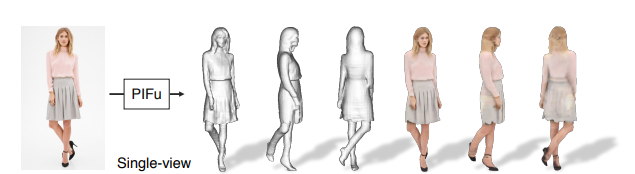
\includegraphics[scale=0.7]{imagenes/antecedentes1.png}
	\caption{Pixel-aligned Implicit function (PIFu) [\cite{pifu}].}
	\label{fig:figura7}
\end{figure}
\pagebreak

Inicialmente se entrena un encoder (codificador) que aprenda sobre vectores de características para cada píxel que existe en la imagen teniendo en cuenta el contexto global relativo a su posición, con este vector y una profundidad en el eje z especificada a lo largo del rayo de cámara saliente del píxel, este aprende a partir de una función implícita que puede clasificar si un punto 3D correspondiente a esta profundidad z está dentro o fuera de la superficie, que en nuestro caso es el cuerpo de una persona.

\subsection{Reconstrucción de la superficie}

Para realizar una buena reconstrucción de manera eficiente en PIFu utiliza una función implícita para definir así la superficie, esta función consiste en un codificador $g$ de imágenes totalmente convolucional y una función $f$ continua e implícita representada por una red MLP (multi-layer perceptrons), donde la superficie esta definida como un conjunto de nivel de:
\begin{equation}
	\label{eq:1}
	f(F(x), z(X)) = s : s \in \mathbb{R}
\end{equation}
Donde para un punto 3D $X$, $x = \pi(X)$ es su proyección 2D, $z(X)$ es el valor de profundidad en el espacio de coordenadas de la cámara, $F(x) = g(I(x))$ es la característica de la imagen en $x$. Se obtiene la función de alineamiento $F(X)$ usando un muestreo bilineal, porque la proyección 2D de $X$ se define en un espacio continuo en lugar de uno discreto (es decir, píxel).
El punto principal de esta función implícita es que aprende a partir del espacio 3D con las características de los píxeles alineados en vez de aprender según las características globales, además esta función se puede presentar como un marco general que puede ser extendido a otras cosas, como por ejemplo predecir los colores RGB.


\begin{figure}[H]
	\centering
	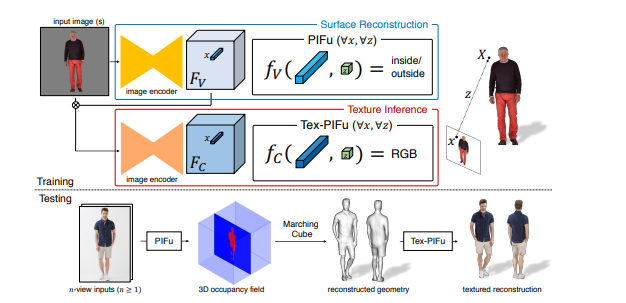
\includegraphics[scale=0.7]{imagenes/antecedentes2.png}
	\caption{Pipeline usada en (PIFu) [\cite{pifu}]. Dada una imagen, PIFu predice la probabilidad continua interior/exterior de un cuerpo humano vestido. Tex-PIFu infiere un valor RGB dados los puntos 3D de la superficie con  con topología arbitraria}
	\label{fig:figura8}
\end{figure}

 Para la reconstrucción de la superficie, se representa como un conjunto de nivel de 0,5 dentro de un campo continuo 3D:
 \begin{equation}
 	\label{eq:2}
 	f_{v}^{*} = \begin{cases}
 				1\text{,}  & \text{X esta dentro de la superficie de la malla}\\
 				0\text{,}  & \text{resto de casos}\\
 			\end{cases}
 \end{equation}

Se entrena la función implícita que alinea píxeles $f_{v}$ minimizando la media del mean squared error (MSE):

\begin{equation}
	\label{eq:3}
	\mathcal{L}_{V} = \frac{1}{n} 
	\sum_{i=1}^{n} | f_{v} (F_{V}(x_{i}) z(X_{i})) - f_{v}^{*}(X_{i}) |^{2}
\end{equation}
 
Donde $X_{i} \in \mathbb{R}^{3}$, $F_{V}(x) = g(I(x))$ es la característica de la imagen del codificador de imágenes $g$ en $x = \pi(X)$ y $n$ es el número de puntos muestrados. Dadas una imagen y la malla 3D correspondiente a la imagen que está espacialmente alineada con la imagen, los parámetros del codificador $g$ y de PIFu $f_{v}$ se actualizan unidas minimizando con la ecuación \ref{eq:3} como [\cite{eq3}] demuestra, el entrenamiento de un codificador de imágenes con un subconjunto de píxeles no le hace daño a la convergencia en comparación a entrenarlo con todos los píxeles[\cite{pifu}]. 

Durante la obtención de la superficie, se muestrea el campo de probabilidad sobre el espacio 3D y se extrae la iso-superficie el campo de probabilidad con un umbral de 0.5 utilizando Marching Cube. 

Este método permite el muestreo directo de puntos 3D sobre la marcha desde la malla en la resolución original utilizando un algoritmo de trazado de rayos eficiente.

\subsection{Obtención de la Textura}
Para la obtención de la textura de la imagen para el modelo 3D, PIFu nos permite predecir de manera directa los colores RGB en la superficie $s$ en la ecuación \ref{eq:4} como un vector con la información de los 3 valores RGB. Sin embargo, extender PIFu a la predicción de colores no es una tarea trivial, ya que los colores están solo definidos en la superficie a diferencia en la reconstrucción tenemos en cuenta todo el espacio 3D. 

Dado unos puntos 3D muestreados en la superficie $X \in \omega$, la función objetivo para la inferencia de textura es el promedio de la función L1 error de los colores como se puede ver en la siguiente ecuación:

\begin{equation}
	\label{eq:4}
	\mathcal{L}_{C} = \frac{1}{n} 
	\sum_{i=1}^{n} | f_{c} (F_{C}(x_{i}) z(X_{i})) - C(X_{i}) |
\end{equation}

Donde $C(X_{i}$ es la verdad básica de los valores de los colores RGB en el punto de superficie $(X_{i} \in \omega$ y $n$ es el numero de puntos muestreados. El problema es que se observó que $f_{c}$ con la función de pérdidas sufría overfitting, esto es provocado porque $f_{c}$ no solo aprende los colores en la superficie sino que también las fronteras de las superficies 3D del objeto por eso $f_{c}$ puede obtener la textura de las  superficies que no se ven con una pose y forma diferente durante la obtención, lo que supone un gran desafío. Para solucionar este problema se realizaron varios cambios, el primero es que la condiciona el codificador de imágenes para la obtención de texturas con las características de la imagen aprendidas en la reconstrucción de la superficie $F_{V}$, con esto el codificador puede enfocarse en la obtención del color dada una geometría incluso los objetos invisibles tienen diferentes formas, poses o topología. Por otro lado se introduce un offset $\epsilon \sim \mathcal{N}(0, d)$ para los puntos de la superficie sobre la superficie normal $N$ así el color puede ser definido no solo por la superficie exacta si no que por el alrededor de este. Con esas modificaciones la función queda así:

\begin{equation}
	\label{eq:5}
	\mathcal{L}_{C} = \frac{1}{n} 
	\sum_{i=1}^{n} | f_{c} (F_{C}(x_{i}^{'}, F{V}), X_{i,z}^{'}) - C(X_{i}) |
\end{equation}

Donde $ X_{i}^{'} = X_{i} + \epsilon$. Se usa un $d = 1.0$ cm para todos los experimentos.

\section{Cálculo de distancias}

Dado que se necesita saber cuán capaz es de representar la realidad este método se necesita realizar una serie de comparaciones, para ello vamos a utilizar dos métodos diferentes.

\subsection{Distancia Chamfer}
Por un lado tenemos la distancia de Chamfer es una métrica de evaluación, en este caso la aplicaremos sobre dos nubes de puntos (la obtenida por nuestro método y la del proyecto de Tech4diet[\cite{tech}]). Tiene en cuenta la distancia de cada punto. Para cada punto en cada nube, esta distancia calcula el punto más cercano en el otro conjunto de puntos y suma el cuadrado de la distancia. [\cite{linyi_2022}]

\begin{equation}
	\label{eq:6}
	CD(S_{1}, S_{2}) = 
	\frac{1}{S_{1}} \sum_{x \in S_{1}}{} \min_{x \in S_1}|| x - y ||_{2}^{2} +
	\frac{1}{S_{2}} \sum_{y \in S_{1}}{} \min_{x \in S_1}|| x - y ||_{2}^{2}
\end{equation}

Donde $S_{1}$ y $S_{2}$ son las dos nubes de puntos y $x$ e $y$ son sus correspondientes puntos.

\subsection{Distancia Hausdorff}
Por otro lado tenemos la distancia de Hausdorff que al igual que la de Chamfer es una métrica de evaluación, esta es la distancia más larga de un conjunto de puntos vecino en el otro conjunto [\cite{grégoire_bouillot_2022}].

\begin{equation}
	\label{eq:7}
	h(S_{1}, S_{2}) = 
	\max_{a \in S_{1}} [ \min_{b \in S_{2}} [d(a,b)]]
\end{equation}

Donde $a$ y $b$ son los puntos de los conjuntos $S_{1}$ y $S_{2}$ respectivamente y $d(a,b)$ es cualquier métrica entre esos dos puntos, esta puede ser la distancia euclídea o cualquier otra.

	% Plantilla: Se muestran listas
%\input{capitulos/objetivos}		% Plantilla: Se muestran tablas
%\input{capitulos/metodologia}	% Plantilla: Se muestran figuras
%\input{capitulos/desarrollo}		% Plantilla: Se muestran listados
%%%%%%%%%%%%%%%%%%%%%%%%%%%%%%%%%%%%%%%%%%%%%%%%%%%%%%%%%%%%%%%%%%%%%%%%%
% Plantilla TFG/TFM
% Escuela Politécnica Superior de la Universidad de Alicante
% Realizado por: Jose Manuel Requena Plens
% Contacto: info@jmrplens.com / Telegram:@jmrplens
%%%%%%%%%%%%%%%%%%%%%%%%%%%%%%%%%%%%%%%%%%%%%%%%%%%%%%%%%%%%%%%%%%%%%%%%

\chapter{Experimentación}
\label{experimentacion}

En este punto del trabajo se va a mostrar toda la experimentación realizada en este proyecto con la red, para ello se va a comenzar comentando los arreglos que se hicieron necesarios para poder realizar la comparación de los modelos.

\section{Limpieza a los modelos obtenidos con la herramienta Tech4diet}

Los modelos generados por Tech4diet, tienen suciedad en la parte de los pies, pues representan la plataforma que pisas para hacerte la reconstrucción del cuerpo.

Este proceso fue necesario para tratar de tener una buena comparativa de modelos obtenidos por nuestra red, dado que hasta la alineación era compleja por este motivo. El proceso se realizó con la herramienta de Blender, se eliminaron las partes sobrantes como se puede ver en la siguiente imagen.

\begin{figure}[H]
	\centering
	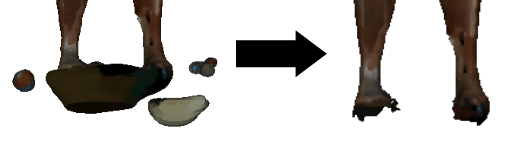
\includegraphics[scale=1]{imagenes/experimentacion1.png}
	\caption{Proceso limpieza modelo Tech4diet}
	\label{fig:figura9}
\end{figure}

Como se puede ver en la figura \ref{fig:figura9} se ha limpiado la plataforma, que no forma parte de nuestro cuerpo.


\section{Alineamiento de modelos}

La distancia de Hausdorff se va a calcular en MeshLab, para realizarla necesitamos alinear los modelos.

Este proceso se hace mediante la herramienta $Align$ dentro de MeshLab, de esta manera, aparece una ventana y alinearemos eligiendo $Point Based Glueling$, para ello antes se selecciona el modelo obtenido por Tech4diet y seleccionamos a $Glue Mesh Here$, esto se hace así porque es la que no queremos que cambie ni de ángulo ni nada en general.

Una vez seleccionada la opción para alinear nos saldrá una ventana en la que iremos eligiendo puntos en ambos modelos para poder alinearlos correctamente.

\begin{figure}[H]
	\centering
	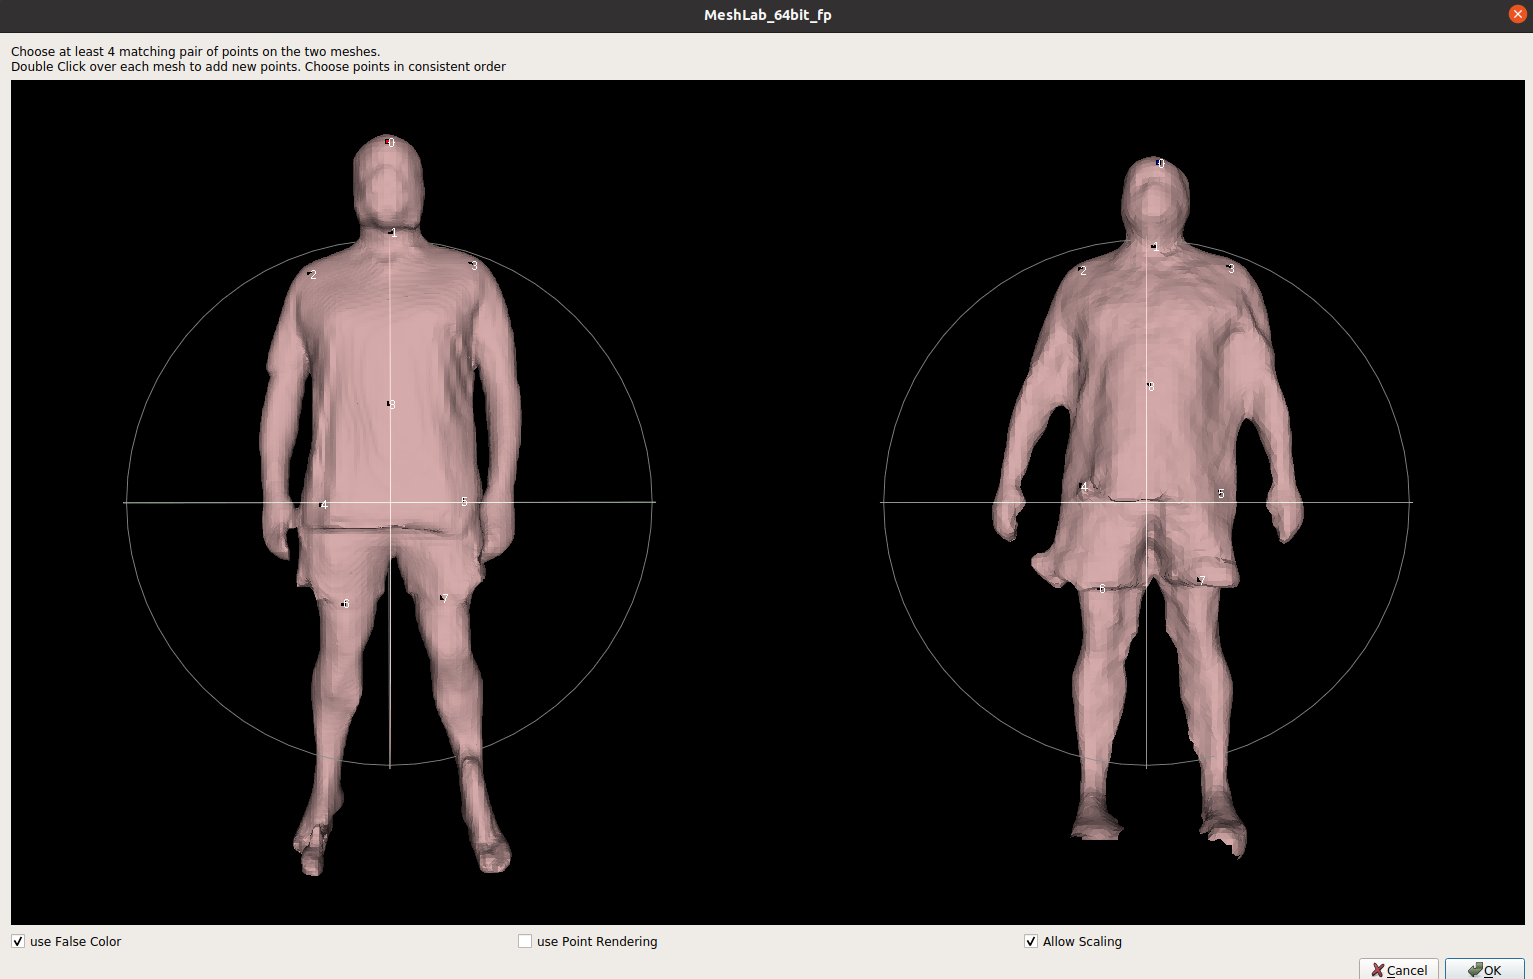
\includegraphics[scale=0.3]{imagenes/alineamiento.png}
	\caption{Proceso alineamiento modelos}
	\label{fig:figura10}
\end{figure}

En la figura \ref{fig:figura10} podemos observar dos modelos, el de la izquierda es el obtenido mediante la red, el de la derecha es el obtenido por Tech4diet

Una vez seleccionados los puntos correctamente y en estos caso seleccionado $Allow Scaling$ (esto lo he hecho porque la red no es capaz de que las medidas sean exactas a diferencia de Tech4diet), se realiza el alineamiento.

\begin{figure}[H]
	\centering
	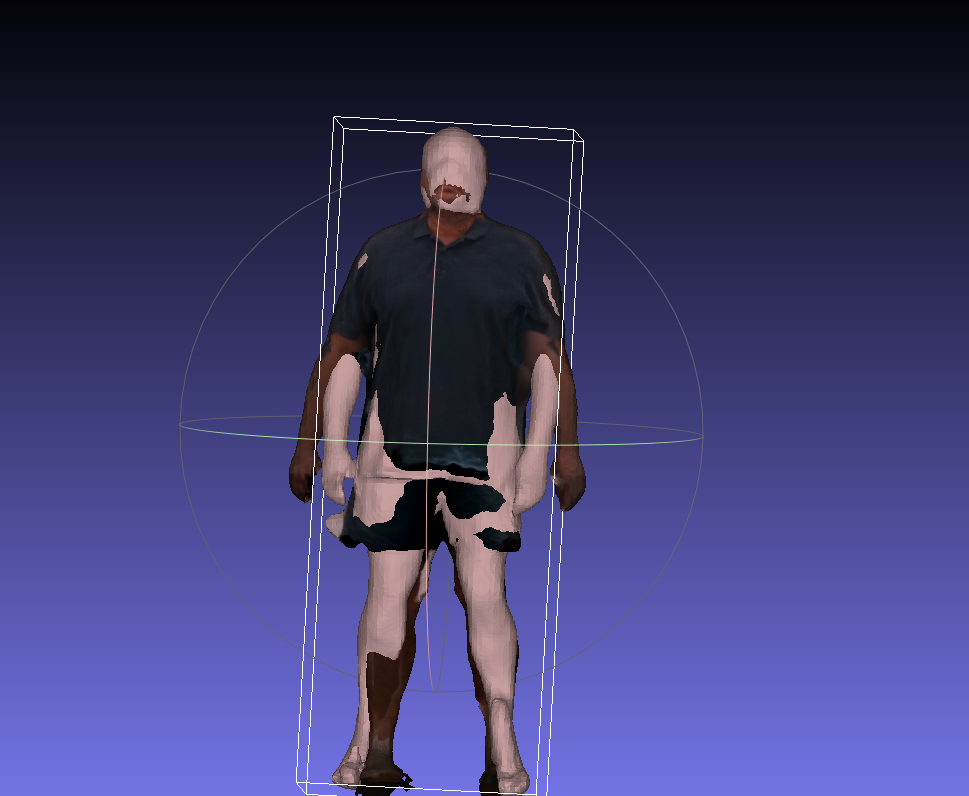
\includegraphics[scale=0.3]{imagenes/alineamiento2.png}
	\caption{Modelos alineados}
	\label{fig:figura11}
\end{figure}

En la figura \ref{fig:figura11} se observa el resultado obtenido después de la alineación.

Con la alineación realizada ya se puede usar la herramienta que nos calcula la distancia de Hausdorff.

\section{Creación de las nubes de punto correspondientes a cada modelo}

Para poder realizar el cálculo de la distancia de Chamfer es necesario tener las nubes de punto, porque las nubes de punto son $arrays$ con las coordenadas (también tienen la información del color y las normales, pero en este caso se va a eliminar esta información). Para ello se puede usar las aplicaciones MeshLab o CloudComparer.

He seleccionado CloudComparer, porque podías eliminar la información de los colores y de las normales desde la misma herramienta.

\section{Cálculo distancias}

Para poder comparar los modelos se han utilizado las distancias de Hausdorff y Chamfer como se ha mencionado con anterioridad, en este punto se va a explicar como se han obtenido las medidas.

\subsection{Distancia Hausdorff}
Como se ha comentado en el punto 4.1, la distancia de Hausdorff de ha calculado mediante la herramienta de MeshLab que te permite calcularla, esta te da un resultado parecido al siguiente: 

\begin{python}
	"Hausdorff Distance computed
	Sampled 58888 pts (rng: 0) on result_camelia0.obj searched closest on Camelia.obj
	min : 0.000000 max 0.339742 mean : 0.020914 RMS : 0.029951
	Values w.r.t. BBox Diag (1.819615)
	min : 0.000000 max 0.186711 mean : 0.011493 RMS : 0.016460"
\end{python}

Donde $min$ dignifica la mínima distancia que hay entre las mallas, $max$ la máxima distancia existente de un punto a otro de las mallas, $mean$ es la media y $RMS$ significa Root Mean Square, que es la raíz cuadrada de la media aritmética de los cuadrado de los valores.

Tenemos dos líneas de valores en la primera esta sobre la unidad de medida que en este caso es en metros, y la segunda línea son los valores anteriores obtenidos pero divididos por la longitud de la diagonal de la bounding box (cuadro delimitador de las mallas) de la malla que se usa como referencia, en este caso usamos la malla obtenida por Tech4diet.

\pagebreak
\subsection{Distancia Chamfer}
Por otro tenemos la distancia Chamfer, para ello se ha programado utilizado la siguiente función en python:

\begin{lstlisting}[caption={Código obtención distancia chamfer}, label=cod:3]
\end{lstlisting}
\begin{python}
	def chamfer_distance(x, y, metric='l2'):
		x_nn = NearestNeighbors(n_neighbors=1, leaf_size=1, algorithm='kd_tree', metric=metric).fit(x)
		min_y_to_x = x_nn.kneighbors(y)[0]
		y_nn = NearestNeighbors(n_neighbors=1, leaf_size=1, algorithm='kd_tree', metric=metric).fit(y)
		min_x_to_y = y_nn.kneighbors(x)[0]
		chamfer_dist = np.mean(min_y_to_x) + np.mean(min_x_to_y)
	return chamfer_dist
\end{python}

En el código \ref{cod:3} se calcula la distancia media mínima para cada punto que hay de la malla $x$ a la $y$ y viceversa.
\clearpage

\section{Comparativas}

Por un lado comentar que la red genera modelos del mismo tamaño sin importar la altura de la persona, este caso es importante y necesario que los tamaños sean los reales, por eso en la herramienta de alineamiento se seleccionó el escalado, pero a diferencia de eso, en la distancia de Chamfer no se ha podido mantener dicho escalado.

\begin{figure}[H]
	\centering
	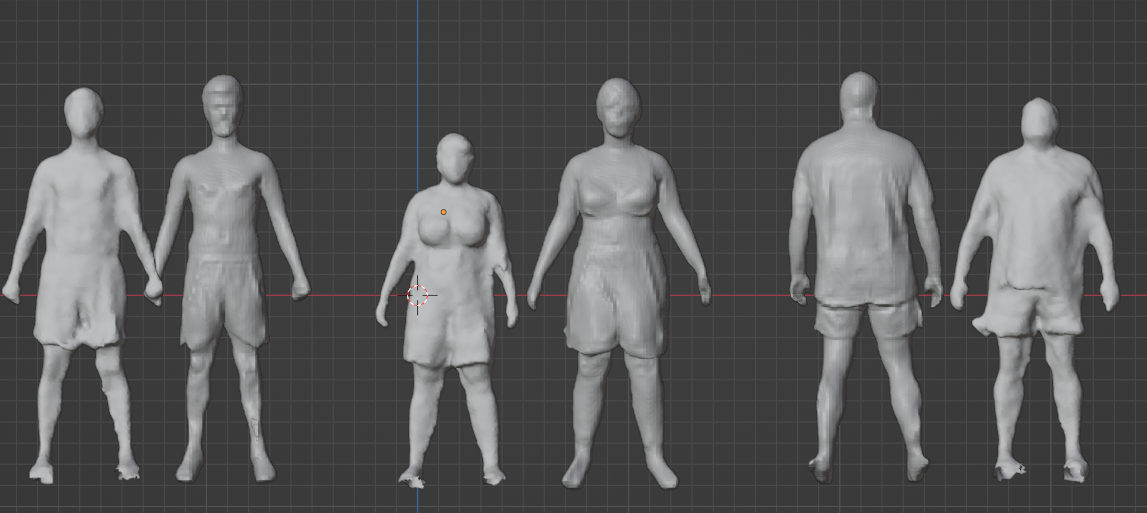
\includegraphics[scale=0.4]{imagenes/difaltura.png}
	\caption{Diferencia de altura de los modelos, el modelo más grande es el generado por la red}
	\label{fig:figura12}
\end{figure}






		% Plantilla: Se muestran gráficas
%%%%%%%%%%%%%%%%%%%%%%%%%%%%%%%%%%%%%%%%%%%%%%%%%%%%%%%%%%%%%%%%%%%%%%%%%
% Plantilla TFG/TFM
% Escuela Politécnica Superior de la Universidad de Alicante
% Realizado por: Jose Manuel Requena Plens
% Contacto: info@jmrplens.com / Telegram:@jmrplens
%%%%%%%%%%%%%%%%%%%%%%%%%%%%%%%%%%%%%%%%%%%%%%%%%%%%%%%%%%%%%%%%%%%%%%%%

\chapter{Conclusiones}
\label{conclusiones}
En este capítulo se resaltan las principales conclusiones obtenidas como consecuencia del trabajo desarrollado y a su vez líneas futuras derivadas de este.

\section{Conclusión}

En el presente trabajo se han planteado una serie de objetivos relacionados con la necesidad de generar un modelo 3D del cuerpo humano, con el uso de una cámara de teléfono móvil y con una sola vista. Se ha seleccionado el uso de una cámara de teléfono móvil porque actualmente toda persona adulta tiene uno, y por lo tanto es un sistema muy flexible y portable.

En relación con el primer objetivo planteado se ha realizado una revisión de varios métodos del estado del arte que abordan la obtención de modelos 3D del cuerpo a partir de imágenes 2D, con énfasis en aquellos que utilizan aprendizaje profundo. Analizado el estado del arte se ha valorado que el método más adecuado es PIFu.

Gracias al estudio anterior, el segundo objetivo ya trata sobre el análisis y adaptación del modelo seleccionado. Se puede concluir con que el funcionamiento de la red es complejo, ya que la se basa en funciones continuas e implícitas (para la reconstrucción de las superficies y para la inferencia de textura) para conseguir los resultados de manera eficiente. Además esta red requiere de parámetros concretos en las imágenes, esto es porque los tensores están preparados para ciertos tamaños, no se puede utilizar cualquier imagen. 

En cuanto el análisis comparativo de la precisión de las medidas obtenidas en los modelos 3D, se ha concluido con que esta red requiere de más información que una vista y que se ha de re-entrenar la red con más tipos de cuerpo, ya que por estas razones las medidas no se acercan tanto a la realidad. Actualmente estos resultados no son viables en el ámbito sanitario.

En referencia al estudio de la red profunda, hemos podido comprobar que la red ha sido alimentada y entrenada por modelos que tienen un físico más normativo, dado que cada vez que se ha probado con un cuerpo menos normativo más errores nos hemos encontrado en el proceso, como por ejemplo una pérdida de peso considerable en comparación cuando observabas los modelos en ángulos más ladeados.

Por último, respecto al estudio de los resultados obtenidos se concluye con que hay ciertos ángulos que favorecen a la red, hemos podido comprobar que el ángulo donde se ve la espalda nos ha proporcionado modelos con menos problemas. También se han probado con imágenes con ruido, donde se añade un cubo verde para que se confunda con el fondo, y la red ha sido capaz de dar resultados, aun que dependiendo de donde se encontrara este cubo proporcionaba más o menos errores. Igualmente, en la mayoría de las ocasiones la vista del modelo 3D se ve perfecta desde el ángulo de la imagen pero cuando empiezas a mirar el resto de ángulos se ven muchos desperfectos y deformidades.

\clearpage
\section{Líneas Futuras}

Como consecuencia del trabajo llevado a cabo se han derivado una serie de líneas futuras entre las que podemos destacar:

Ampliación del uso de la red a multivista, ya que como se ha comentado en las conclusiones, se puede observar que el ángulo utilizado en la imagen 2D, se representa bien en el modelo 3D, el problema ocurre una vez se observa desde más ángulos, esto se puede solucionar dándole a la red más información con diferentes ángulos. Además PIFu[\cite{pifu}] es exportable a multivista, por lo que facilita este trabajo.

Entrenamiento con diferentes modelos sobre diferentes tipos de cuerpos humanos para obtener mejores resultados, y prepararlo para multivista, para ello se necesitará un amplio DataSet.

Por último realizar comparaciones de los resultados obtenidos con multivista y una vista.
	% Plantilla: Se muestran matemáticas

%%%%
% CONTENIDO. BIBLIOGRAFÍA.
%%%%
\nocite{*} %incluye TODOS los documentos de la base de datos bibliográfica sean o no citados en el texto
\bibliography{bibliografia/bibliografia2} % Archivo que contiene la bibliografía
\bibliographystyle{apacite}

%%%%
% CONTENIDO. LISTA DE ACRÓNIMOS. Comenta las líneas si no lo deseas incluir.
%%%%
% Incluye el listado de acrónimos utilizados en el trabajo. 
%\printglossary[style=modsuper,type=\acronymtype,title={Lista de Acrónimos y Abreviaturas}]
% Añade el resto de acrónimos si así se desea. Si no elimina el comando siguiente
%\glsaddallunused 

%%%%
% CONTENIDO. Anexos - Añade o elimina según tus necesidades
%%%%
%\appendix % Inicio de los apéndices
%%%%%%%%%%%%%%%%%%%%%%%%%%%%%%%%%%%%%%%%%%%%%%%%%%%%%%%%%%%%%%%%%%%%%%%%%
% Plantilla TFG/TFM
% Escuela Politécnica Superior de la Universidad de Alicante
% Realizado por: Jose Manuel Requena Plens
% Contacto: info@jmrplens.com / Telegram:@jmrplens
%%%%%%%%%%%%%%%%%%%%%%%%%%%%%%%%%%%%%%%%%%%%%%%%%%%%%%%%%%%%%%%%%%%%%%%%

\chapter{Anexo I}
\label{anexos}

\section{Anexo 1}
\subsection{Gráficas del cálculo de distancias del modelo 1}
\begin{figure}[H]
	\centering
	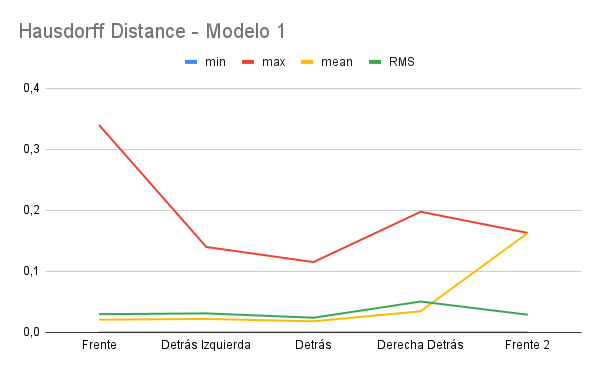
\includegraphics[scale=0.55]{imagenes/Hausdorff-M1.png}
	\caption{Gráfica sobre los cálculos obtenidos con Hausdorff y el modelo 1 comparado con los modelos en diferentes ángulos obtenidos con la red PIFu[\cite{pifu}]}
	\label{fig:figura14}
\end{figure}

\begin{figure}[H]
	\centering
	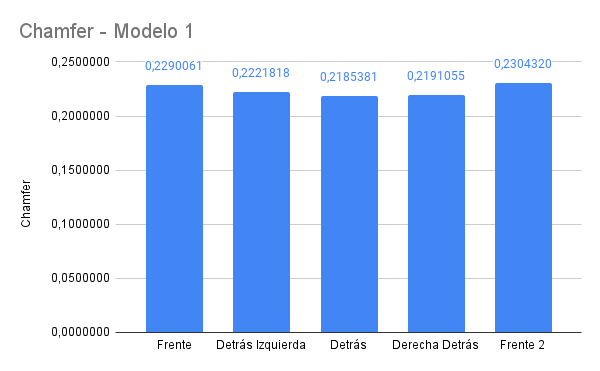
\includegraphics[scale=0.55]{imagenes/Chamfer-M1.png}
	\caption{Gráfica sobre los cálculos obtenidos con Chamfer y el modelo 1 comparado con los modelos en diferentes ángulos obtenidos con la red PIFu[\cite{pifu}]}
	\label{fig:figura15}
\end{figure}
\subsection{Gráficas del cálculo de distancias del modelo 2}
\begin{figure}[H]
	\centering
	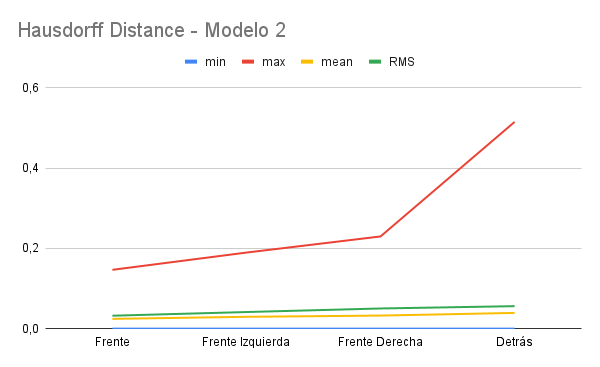
\includegraphics[scale=0.55]{imagenes/Hausdorff-M2.png}
	\caption{Gráfica sobre los cálculos obtenidos con Hausdorff y el modelo 2 comparado con los modelos en diferentes ángulos obtenidos con la red PIFu[\cite{pifu}]}
	\label{fig:figura16}
\end{figure}

\begin{figure}[H]
	\centering
	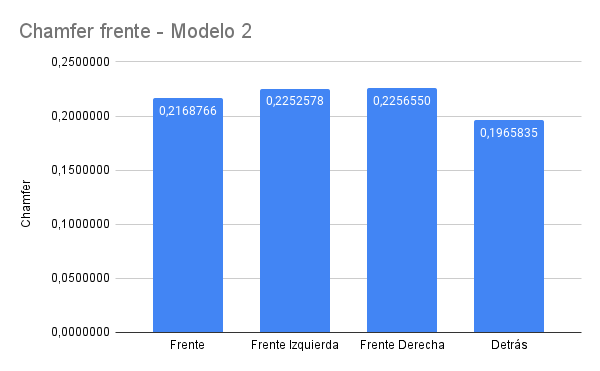
\includegraphics[scale=0.55]{imagenes/Chamfer-M2.png}
	\caption{Gráfica sobre los cálculos obtenidos con Chamfer y el modelo 2 comparado con los modelos en diferentes ángulos obtenidos con la red PIFu[\cite{pifu}]}
	\label{fig:figura17}
\end{figure}
\subsection{Gráficas del cálculo de distancias del modelo 3}
\begin{figure}[H]
	\centering
	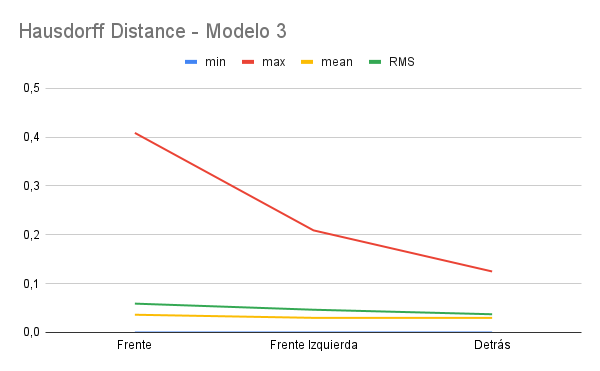
\includegraphics[scale=0.55]{imagenes/Hausdorff-M3.png}
	\caption{Gráfica sobre los cálculos obtenidos con Hausdorff y el modelo 3 comparado con los modelos en diferentes ángulos obtenidos con la red PIFu[\cite{pifu}]}
	\label{fig:figura18}
\end{figure}

\begin{figure}[H]
	\centering
	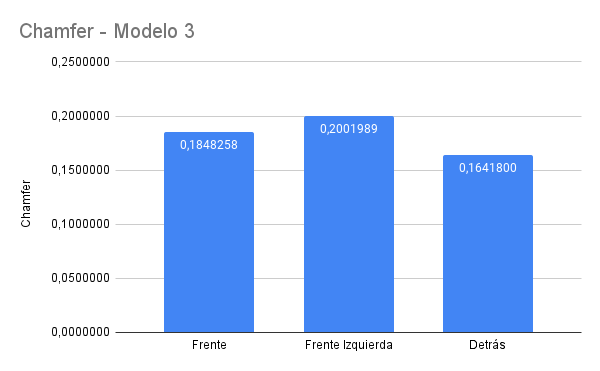
\includegraphics[scale=0.55]{imagenes/Chamfer-M3.png}
	\caption{Gráfica sobre los cálculos obtenidos con Chamfer y el modelo 3 comparado con los modelos en diferentes ángulos obtenidos con la red PIFu[\cite{pifu}]}
	\label{fig:figura19}
\end{figure}


\section{Anexo 2}

\subsection{Modelos con ruido añadido}

\begin{figure}[H]
	\centering
	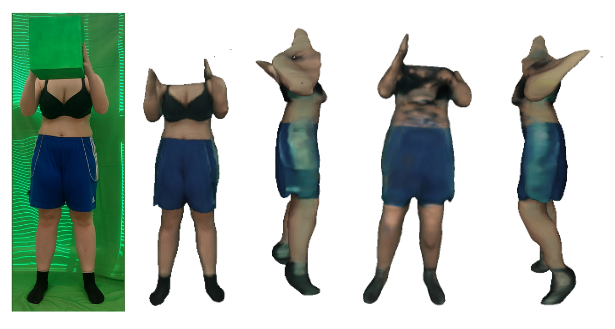
\includegraphics[scale=0.65]{imagenes/cameliae.png}
	\caption{Modelo obtenido con ruido en la cabeza}
	\label{fig:figura20}
\end{figure}

\begin{figure}[H]
	\centering
	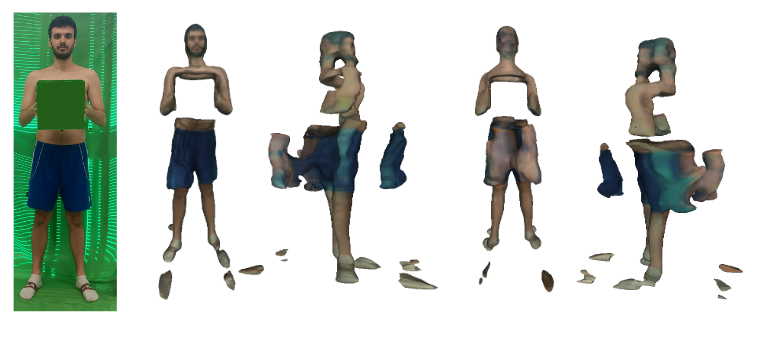
\includegraphics[scale=0.65]{imagenes/nahuele1.png}
	\caption{Modelo obtenido con ruido en el pecho}
	\label{fig:figura21}
\end{figure}

\begin{figure}[H]
	\centering
	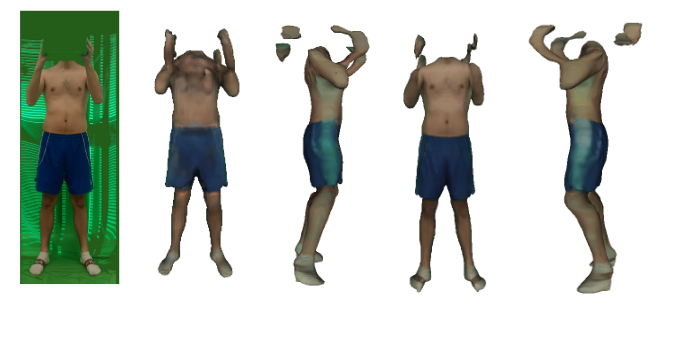
\includegraphics[scale=0.65]{imagenes/nahuele2.png}
	\caption{Modelo obtenido con ruido en la cabeza}
	\label{fig:figura22}
\end{figure}

\section{Anexo 3}

\subsection{Modelo 1}
\begin{figure}[H]
	\centering
	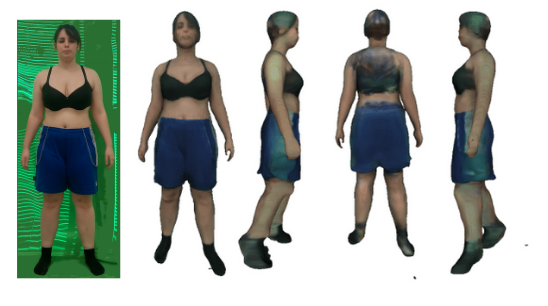
\includegraphics[scale=0.65]{imagenes/camelia0.png}
	\caption{Modelo 1, vista Frente}
	\label{fig:c1}
\end{figure}
\begin{figure}[H]
	\centering
	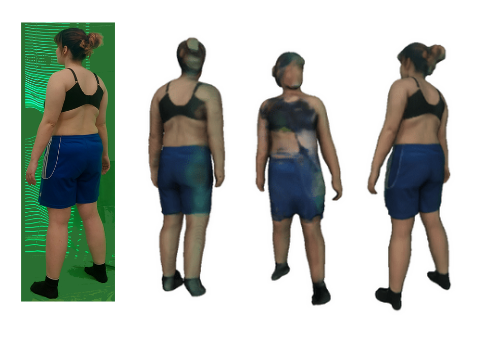
\includegraphics[scale=0.65]{imagenes/camelia5.png}
	\caption{Modelo 1, vista Detrás-Izquierda}
	\label{fig:c2}
\end{figure}
\begin{figure}[H]
	\centering
	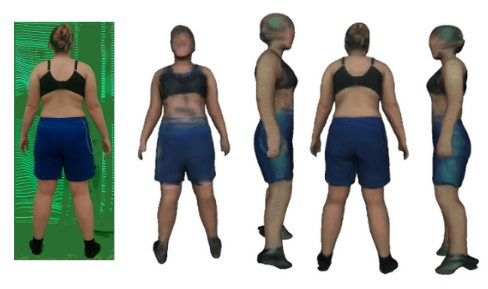
\includegraphics[scale=0.65]{imagenes/camelia6.png}
	\caption{Modelo 1, vista Detrás}
	\label{fig:c3}
\end{figure}
\begin{figure}[H]
	\centering
	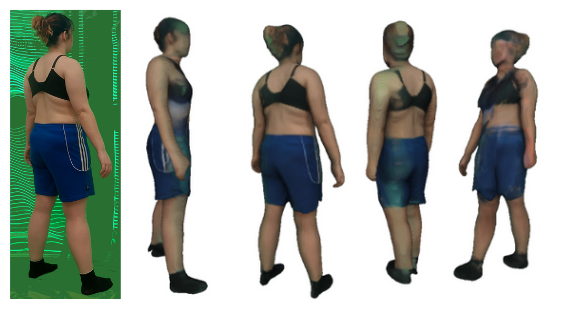
\includegraphics[scale=0.65]{imagenes/camelia7.png}
	\caption{Modelo 1, vista Detrás-Derecha}
	\label{fig:c4}
\end{figure}
\begin{figure}[H]
	\centering
	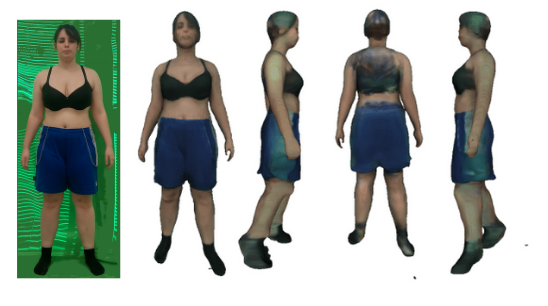
\includegraphics[scale=0.65]{imagenes/camelia0.png}
	\caption{Modelo 1, vista Frente 2}
	\label{fig:c5}
\end{figure}

\subsection{Modelo 2}
\begin{figure}[H]
	\centering
	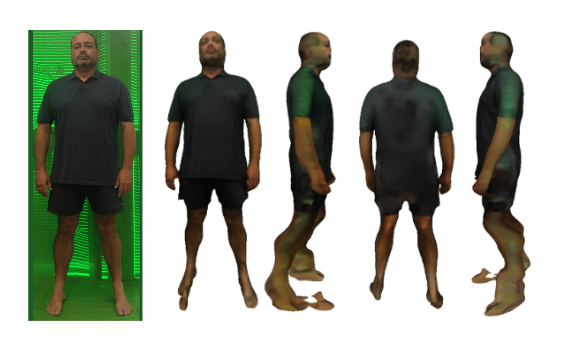
\includegraphics[scale=0.65]{imagenes/andres1.png}
	\caption{Modelo 2, vista Frente}
	\label{fig:a1}
\end{figure}
\begin{figure}[H]
	\centering
	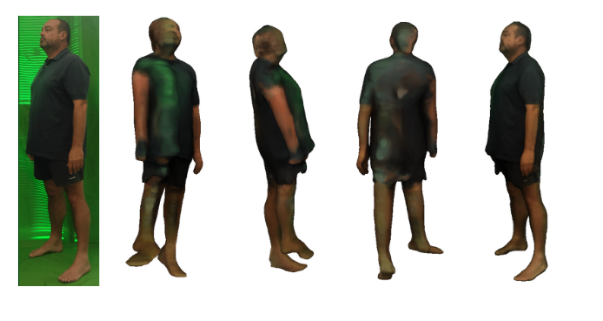
\includegraphics[scale=0.65]{imagenes/andres2.png}
	\caption{Modelo 2, vista Frente-Izquierda}
	\label{fig:a2}
\end{figure}
\begin{figure}[H]
	\centering
	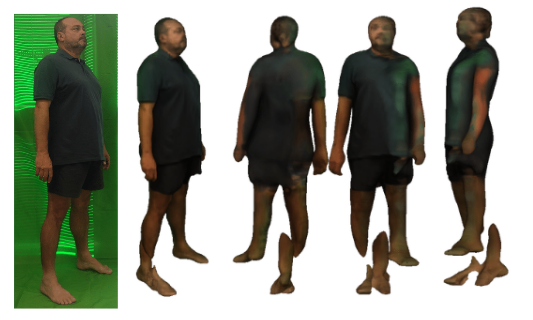
\includegraphics[scale=0.65]{imagenes/andres3.png}
	\caption{Modelo 2, vista Frente-Derecha}
	\label{fig:a3}
\end{figure}
\begin{figure}[H]
	\centering
	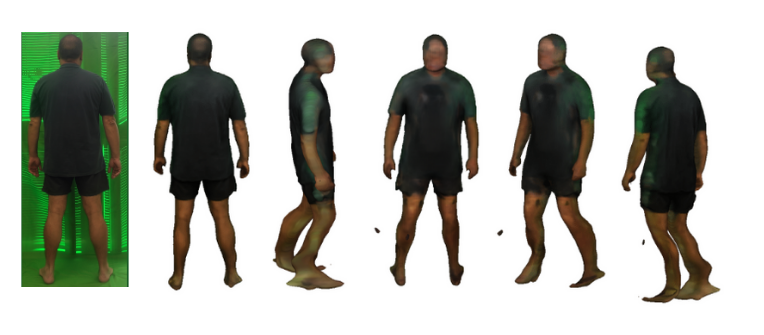
\includegraphics[scale=0.65]{imagenes/andres4.png}
	\caption{Modelo 2, vista Detrás}
	\label{fig:a4}
\end{figure}
\subsection{Modelo 3}

\begin{figure}[H]
	\centering
	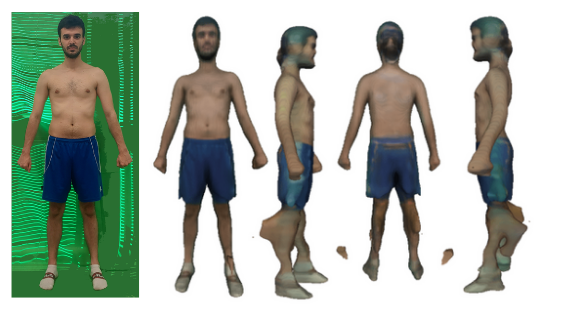
\includegraphics[scale=0.65]{imagenes/nahuel1.png}
	\caption{Modelo 3, vista Frente}
	\label{fig:n1}
\end{figure}
\begin{figure}[H]
	\centering
	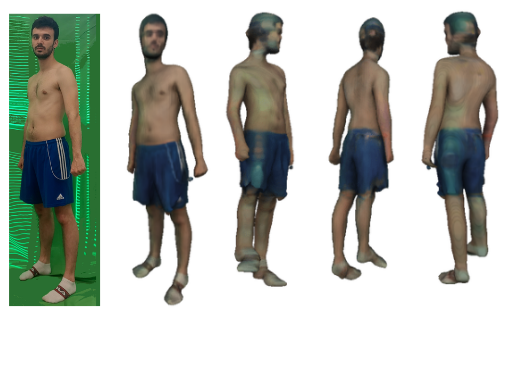
\includegraphics[scale=0.65]{imagenes/nahuel2.png}
	\caption{Modelo 3, vista Frente-Izquierda}
	\label{fig:n2}
\end{figure}
\begin{figure}[H]
	\centering
	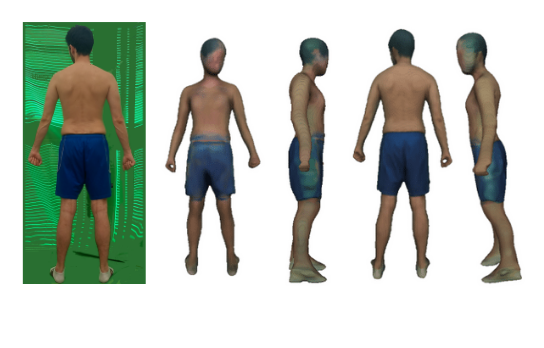
\includegraphics[scale=0.65]{imagenes/nahuel3.png}
	\caption{Modelo 3, vista Detrás}
	\label{fig:n3}
\end{figure}

%\input{anexos/anexo_2}
%\input{anexos/anexo_3}

\end{document}
